\section{Experiments}
\label{sec:experiments}

The experimental evaluation of the proposed method is presented in this section. 
Section \ref{sec:exp_pre} provides details about the custom dataset collected as described in Section \ref{sec:proposed}, as well as preprocessing steps.
Section \ref{sec:exp_transfer} focuses on the transfer learning process of YOLOv8 using the custom dataset.
The experimental results are presented in detail in Section \ref{sec:exp_results}.

\subsection{Custom dataset \& Pre-processing}
\label{sec:exp_pre}
A large-scale custom dataset consisting over 16 hours of data was collected. 
Videos recorded from dashboard cameras during real road driving were utilized, resulting in a total of more than $11,000$ images.
These images were obtained by setting the time interval $T$ to $5$ seconds.
Manual annotation was performed on all images to label the bounding box of the driving vehicle and the brake light status of each vehicle.
The total number of annotations exceeded $30,000$.
To ensure a balanced and diverse dataset, various driving scenarios were included, such as daytime, nighttime, city, highway, and tunnel environments.
Precautions were taken to avoid bias toward any specific category, ensuring information about the number of images and annotations in the train and test sets for each category of brake light status.
The details of numbers of images and annotations in the train and test sets in each category of brake light status are given in Table \ref{tab:dataset}.

\begin{table}[h]
    \caption{Details of train and test datasets}
    \label{tab:dataset}
    % \resizebox{\textwidth*0.5}{!}{%
    \begin{tabular}{p{5cm} p{5cm} p{5cm}}
        % {lrr}
    \toprule
    \multicolumn{1}{c}{Number of}                          & \multicolumn{1}{c}{Train} & \multicolumn{1}{c}{Test} \\
    \midrule
    Images                              & \multicolumn{1}{r}{7,892}                     & \multicolumn{1}{r}{3,196}                    \\
    Annotations                         & \multicolumn{1}{r}{19,913}                    & \multicolumn{1}{r}{10,531}                   \\
    \multicolumn{1}{c}{Brake Light Off ($C_{1}=1.0$)} & \multicolumn{1}{r}{10,851}                    & \multicolumn{1}{r}{5,999}                    \\
    \multicolumn{1}{c}{Brake Light On ($C_{2}=1.0$)}  & \multicolumn{1}{r}{9,062}                     & \multicolumn{1}{r}{4,532}                   \\
    \bottomrule
    \end{tabular}%
    % }
\end{table}

\begin{figure}[b!]%

    \subfloat{{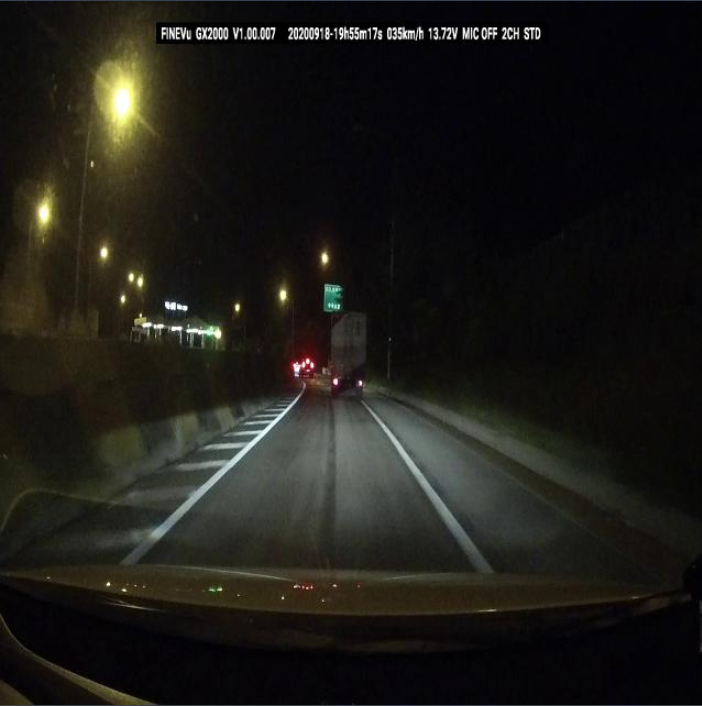
\includegraphics[height=4.5cm]{fig/image20.png} }}%
    \subfloat{{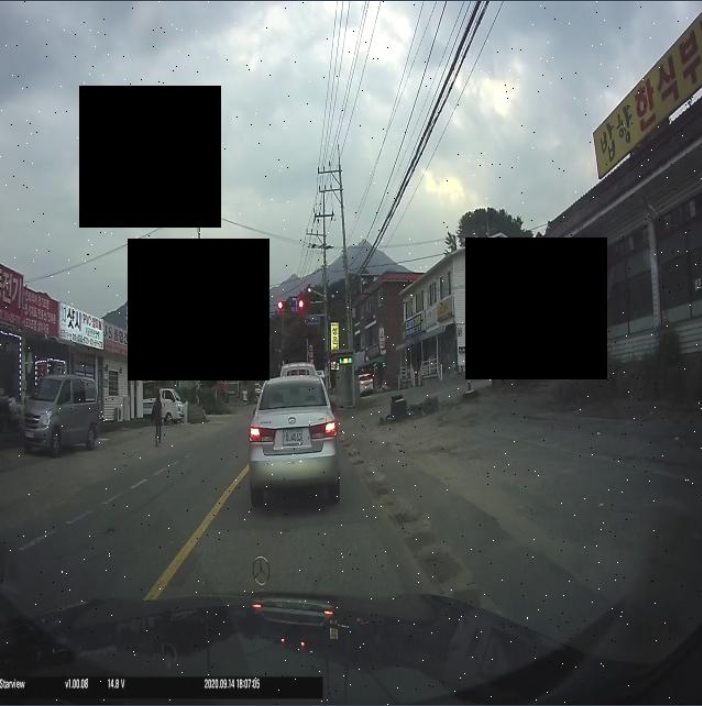
\includegraphics[height=4.5cm]{fig/image21.png} }}%
    \subfloat{{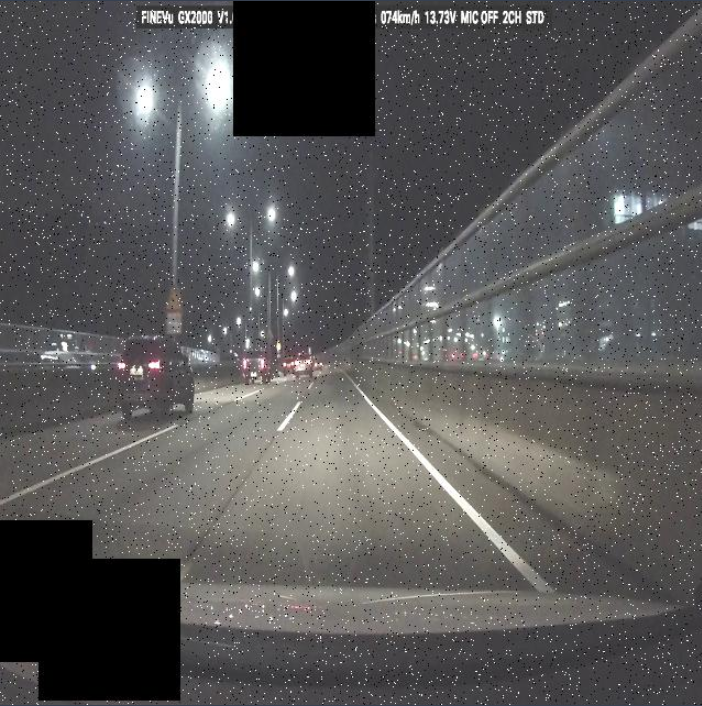
\includegraphics[height=4.5cm]{fig/image22.png} }}%
    \hfill
    \subfloat{{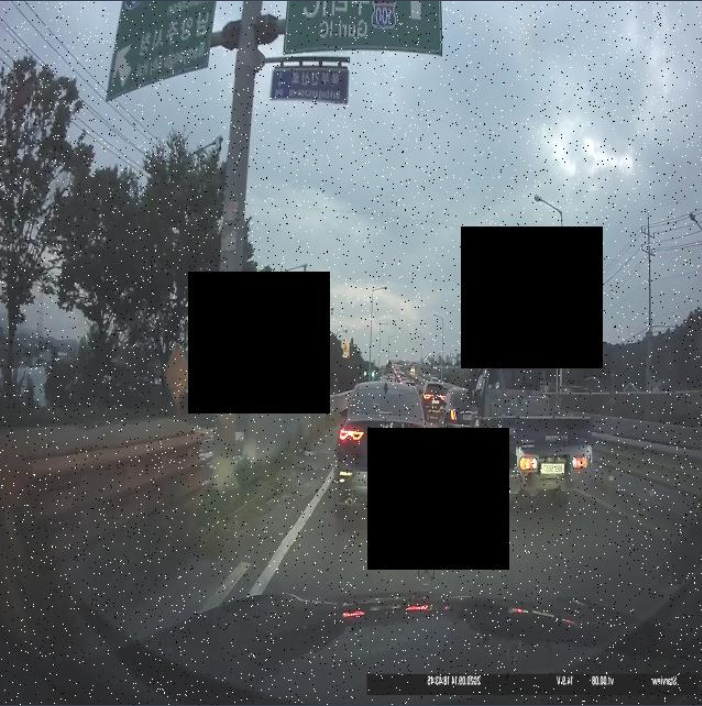
\includegraphics[height=4.5cm]{fig/image23.png} }}%
    \subfloat{{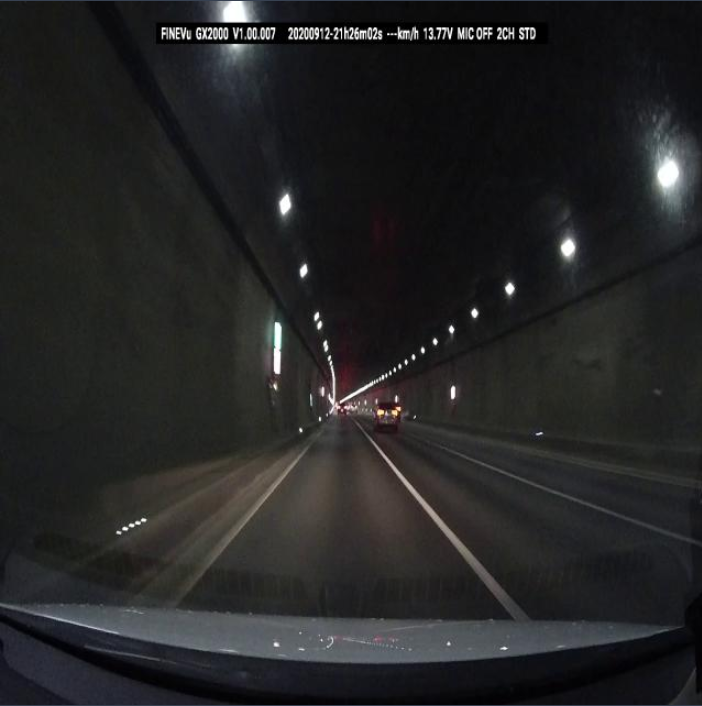
\includegraphics[height=4.5cm]{fig/image24.png} }}%
    \subfloat{{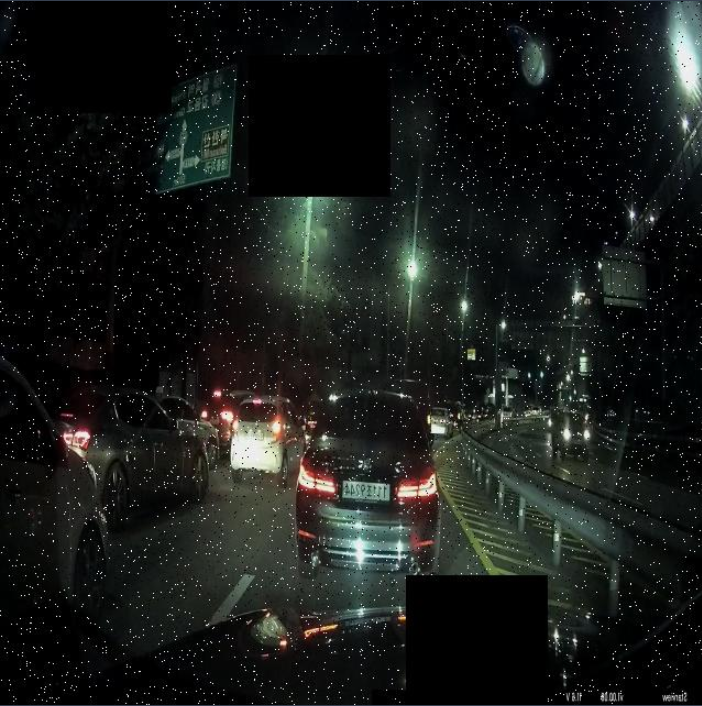
\includegraphics[height=4.5cm]{fig/image25.png} }}%

\caption{Preprocessed input images of custom dataset}
\label{fig:custom_dataset}%
\end{figure}

To make our custom dataset trainable with YOLOv8 and achieve robust performance, several preprocessing steps are necessary.
The first crucial processes involve image resizing and normalization.
In order to maintain a consistent input size, the width and height of all images were resized to $I_{w}$ and $I_{h}$, respectively. 
In this study, both $I_{w}$ and $I_{h}$ were defined as $640$.
Regarding image normalization, min-max normalization was applied to normalize the pixel values.
The normalization precess ensure that all pixel values fall within a specific range, typically between $0$ and $1$, and is performed as follows:

\begin{equation}
    x_{norm} = \frac{x - x_{min}}{x_{max} - x_{min}}
\end{equation}

where $x$ and $x_{norm}$ are origin and normalized pixel value, respectively and $x_{max}$ and $x_{min}$ are the maximum and minimum pixel value of the image, respectively.
In this study, the values for $x_{max}$ and $x_{min}$ were set to $255.0$ and $0.0$, respectively, following the usual convention.
Furthermore, various data augmentation techniques were applied to enhance the robustness of the inference performance.
Random horizontal flipping and image cropping were performed to generate variations of the collected images that could realistically occur.
To improve detection performance in cases of occlusion, random black-box cutout augmentation was also applied.
Finally, to ensure robustness across different camera setups, the quality of the input images was intentionally degraded using various methods.



As stated in Section \ref{sec:method_dataset}, the dashboard cameras used for image acquisition are equipped with various postprocessing methods to captured high-quality images.
to ensure the robust performance of the trained network even with general cameras, random modifications such as brightness changes, blur, and noise injection were applied to the images.
Figure \ref{fig:custom_dataset} provides examples of preprocessed images.
All preprocessing steps were performed using Roboflow \cite{roboflow}, a comprehensive platform for computer vision and image processing tasks.
The preprocessed train dataset is publicly available for access \cite{brake-light-detection_dataset}.



\subsection{Transfer learning}
\label{sec:exp_transfer}
In this study, we conducted transfer learning on all models provided by YOLOv8 \cite{YOLOv8} to develop a detection network that achieves real-time inference in a driving vehicle while maintaining accurate detection.
The YOLOv8 architecture offers five different models of varying sizes, ranging from the smallest model (YOLOv8n) to the largest model (YOLOv8x), as shown in Table \ref{tab:yolov8}.
To ensure consistency, the same set of hyperparameters was applied to all models during training.
A random 20\% of the train dataset was set aside as the validation dataset for monitoring the training progress.
The initial parameter values for each model were obtained from the pretrained parameters officially provided by YOLOv8.
The training process consisted fo $300$ iterations, with a patience value of $20$.
If there was no observable improvement in the validation loss over the most recent $20$ iterations, the training was terminated early to save time and resources.
Stochastic gradient descent (SGD) optimizer with a learning rate of $0.01$ was used, incorporating both momentum and Nesterov Accelerated Gradient (NAG) techniques \cite{sutskever2013importance} with a momentum coefficient of $0.937$.
The training loss was calculated using three loss function: binary cross-entropy, CIoU, and DFL.
The weighting factors assigned th these loss functions were $0.5$, $7.5$, and $1.5$, respectively.
These factors were chosen to balance the impact of each loss function during training.

\begin{table}[h]
    \caption{Official deployed models of YOLOv8}
    \label{tab:yolov8}
    % \resizebox{\textwidth}{!}{%
    \begin{tabular}{lcc}
    \toprule
    \multicolumn{1}{c}{Model}   & \# params (M) & FLOPs (B) \\
    \midrule
    YOLOv8n & 3.2        & 8.7       \\
    YOLOv8s & 11.2       & 28.6      \\
    YOLOv8m & 25.9       & 78.9      \\
    YOLOv8l & 43.7       & 165.2     \\
    YOLOv8x & 68.2       & 257.8     \\
    \bottomrule
    \multicolumn{3}{l}{\textit{Note:} All values in the table correspond}\\
    \multicolumn{3}{l}{\qquad \; to an input image size of 640x640.}
    \end{tabular}%
    % }
\end{table}

\begin{figure}[t]%

    \subfloat{{\includegraphics[height=1.9cm]{fig/Capture/0_highway.jpg} }}%
    \subfloat{{\includegraphics[height=1.9cm]{fig/Capture/0_city.jpg} }}%
    \subfloat{{\includegraphics[height=1.9cm]{fig/Capture/0_tunnel.jpg} }}%
    \subfloat{{\includegraphics[height=1.9cm]{fig/Capture/0_night.jpg} }}%
    \hfill
    \subfloat{{\includegraphics[height=1.9cm]{fig/Capture/0_motor.jpg} }}%
    \subfloat{{\includegraphics[height=1.9cm]{fig/Capture/0_bus.jpg} }}%
    \subfloat{{\includegraphics[height=1.9cm]{fig/Capture/0_truck.jpg} }}%
    \subfloat{{\includegraphics[height=1.9cm]{fig/Capture/0_special_1.jpg} }}%

\caption{Images of driving vehicle and brake light status detection results by proposed networks. Images in the first row depict the detection results in various road environments. From left to right, the depicted environments are highway, city, tunnel, and nighttime. Images in the second row depict the detection results of various vehicle types. From left to right, the depicted vehicle types include motorcycle, bus, trucks, and special vehicle.}
\label{fig:detection}%
\end{figure}




\subsection{Results}
\label{sec:exp_results}
In this section, the evaluation results of the trained detection models are presented, both qualitatively and quantitatively.
Qualitative analysis confirmed that the trained detection models accurately detect the bounding boxes of driving vehicles and classify their brake light status (on or off) in various road environments.
The models demonstrated robust performance in different driving scenarios, including highway, city, tunnel, and nighttime driving.
The qualitative detection results, showcasing the accurate detection of different types of vehicles, including passenger cars, motorcycles, buses, trucks, and special vehicles, are shown in Figure \ref{fig:detection}.

The evaluation of the driving vehicle and brake light status detection performance of each model that underwent transfer learning is conducted by calculating the mean average precision (mAP) on the testset.
Two mAP values are calculated: mAP50 and mAP50-95.
mAP50 represents the average presicion at an intersection over union (IoU) threshold of $0.5$. The IoU threshold measures the overlap between the predicted bounding boxes and the ground truth labels, indicating how well the predicted boxes align with the actual objects.
mAP50-95 represents the average precision over a range of IoU thresholds from $0.5$ to $0.95$, with a step size of $0.05$. 
This metric provides comprehensive assessment of the detection model's performance across different levels of overlap.
Both mAP50 and mAP50-95 are commonly used metrics to evaluate the overall performance of object detection models.

\begin{figure}[t]%

    \subfloat[\centering mAP50 on the entire testset]{{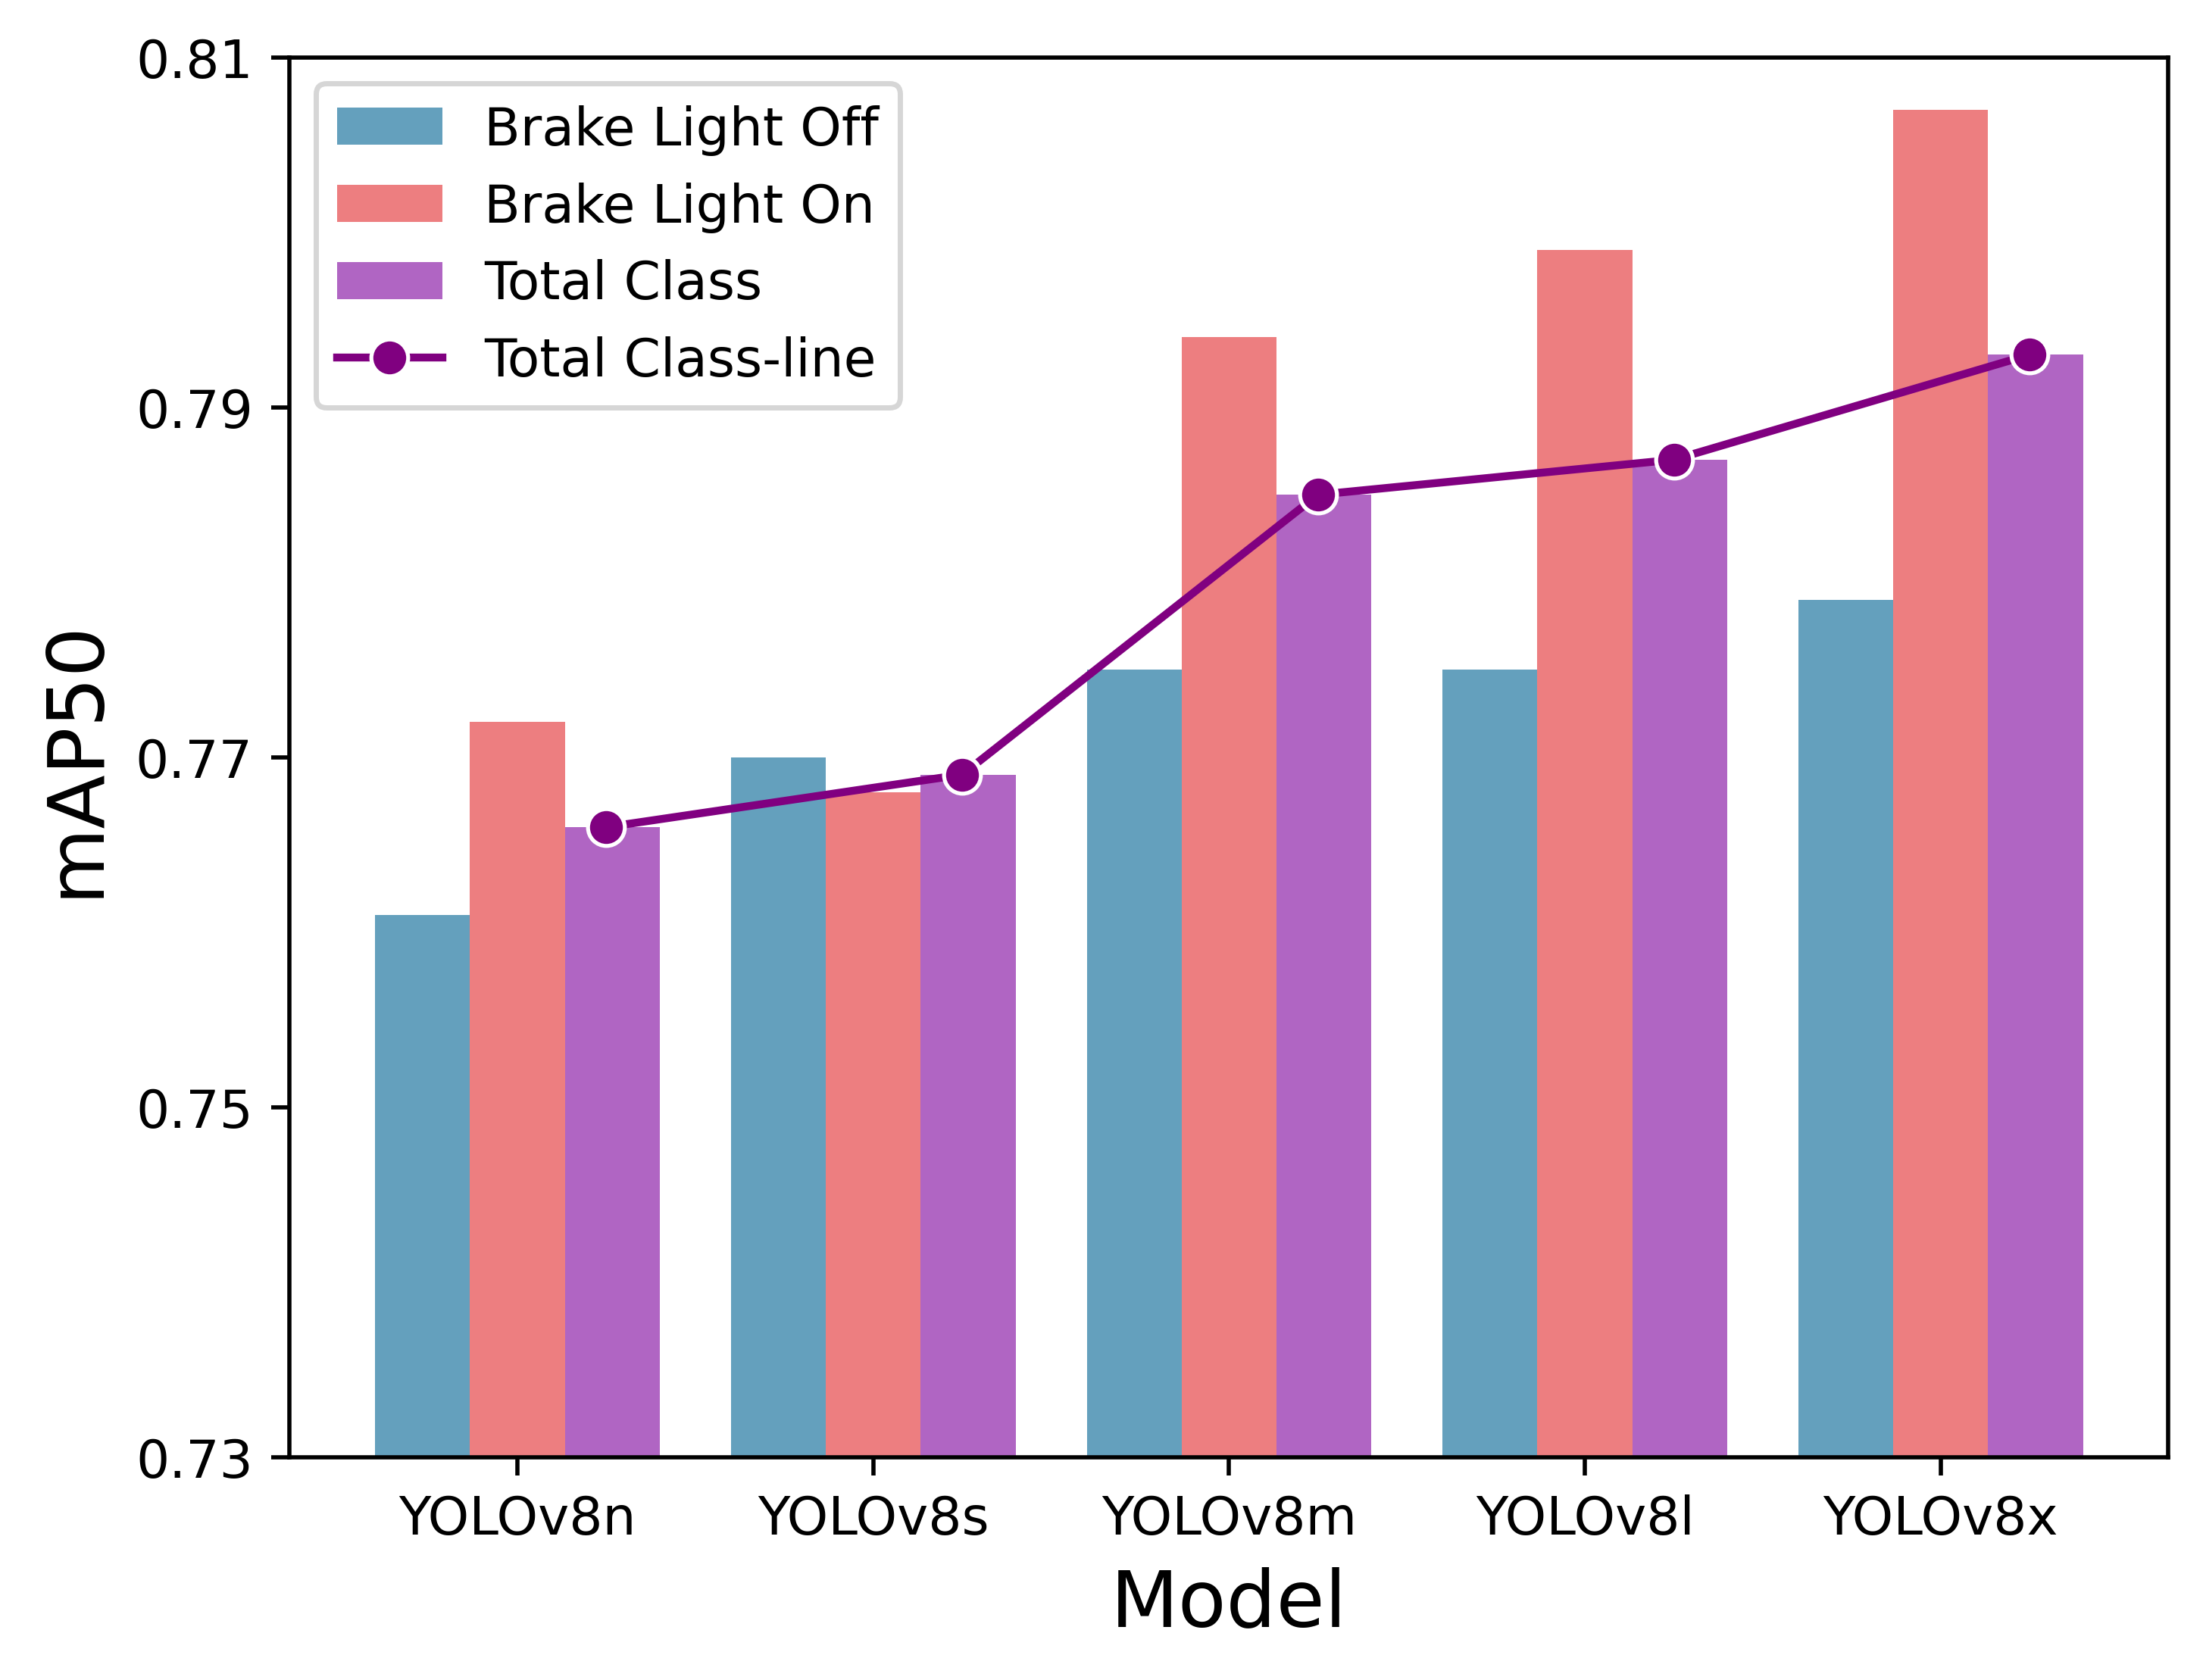
\includegraphics[height=5cm]{fig/bar_map50.png} }}%
    \subfloat[\centering mAP50-95 on the entire testset]{{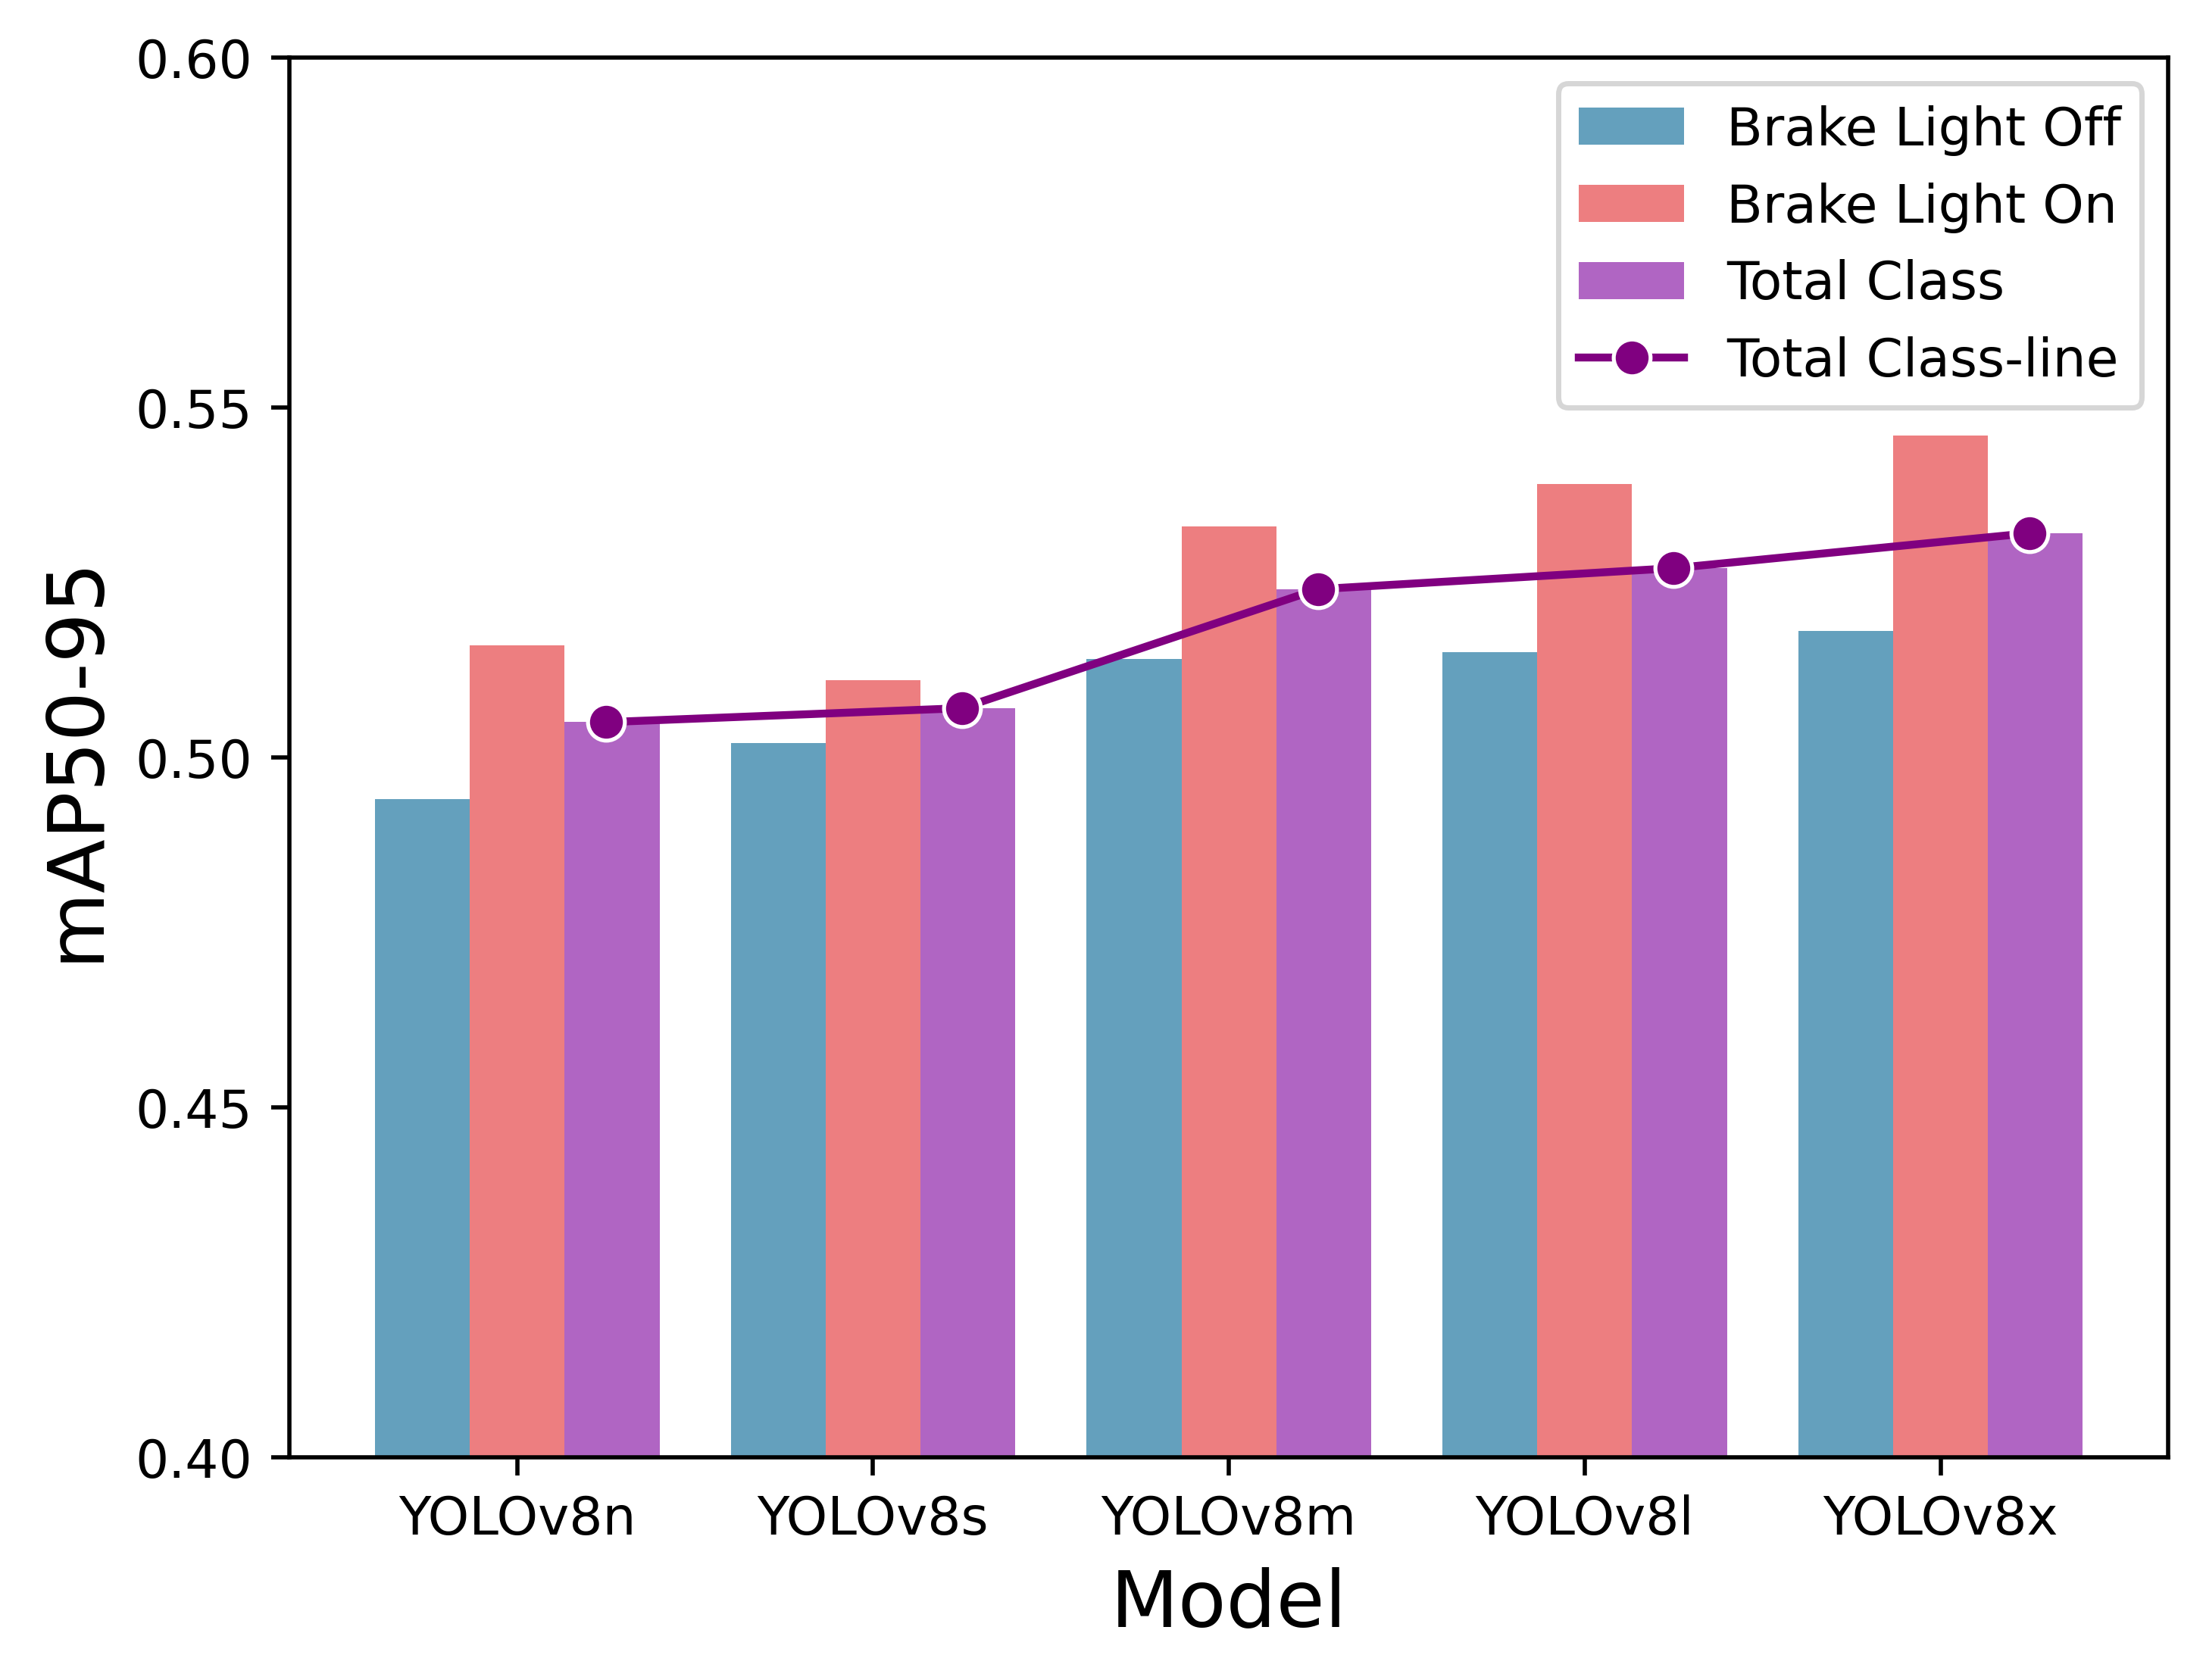
\includegraphics[height=5cm]{fig/bar_map50-95.png} }}%

\caption{Detection performance on the entire testset. The y-axis represents the detection accuracy, and the x-axis lists the YOLOv8 models, with larger models positioned toward the right. Each model is depicted with three bars, showcasing the detection performance for brake light off class, brake light on class, and total class, respectively. Single line plot highlights the difference in detection performance by models for total class.}
\label{fig:test_results}%
\end{figure}



Figure \ref{fig:test_results} presents the detection performance of each trained model, showcasing the results for mAP50 and mAP50-90 in Figure \ref{fig:test_results}-(a) and (b) respectively.
The detection performance for each individual classes, brake light off and brake light on, is represented by blue and red bars respectively. 
The overall detection performance for all classes is shown by the purple bar, with a purple line plot illustrating the trend of performance differences across models.
Both mAP50 and mAP50-95 exhibit similar overall trands, although they differ in scale.
As expected, the detection performance for all classes generally increases as the model size increases.
However, the YOLOv8s model shows a slightly lower performance increase, primarily due to its lower brake light on class detection performance.
Comparing the mAP50 values for each class, it can be observed that all models, except for YOLOv8s, have higher detection performance for the brake light on class compared to the brake light off class.
Overall, the proposed methodology achieved mAP50 values ranging from $0.766$ to $0.793$ and mAP50-95 values ranging from $0.505$ to $0.532$.
Considering the recent benchmarking performance of MS-COCO \cite{lin2014microsoft}, which is one of the leading object detection, with mAP50 values ranging form $71.9$ to $77.0$ and mAP50-95 values ranging from $57.7$ to $58.8$, the proposed methodology demonstrates significant results \cite{coco_benchmark, zou2023object}.
Detailed detection performance for each model and class can be found in Table \ref{tab:total}.

\begin{table}[!h]
    \caption{Results of the entire testset}
    \label{tab:total}
    % \resizebox{\textwidth}{!}{%
    % \begin{tabular}{>{\raggedright}p{2.5cm} >{\raggedright}p{2.5cm} >{\centering}p{2.5cm} >{\centering\arraybackslash}p{2.5cm}}
    \begin{tabular}{llrr}
    \toprule
    \multicolumn{1}{c}{Model} & \multicolumn{1}{c}{Class} & \multicolumn{1}{c}{mAP50} & \multicolumn{1}{c}{mAP50-95} \\
    \midrule
    \multirow{3}{*}{YOLOv8n}  & Brake Light Off           & 0.761                     & 0.494                          \\
                              & Brake Light On            & 0.772                     & 0.516                        \\
                              & \multicolumn{1}{r}{Total} & 0.766                     & 0.505                        \\
    \midrule
    \multirow{3}{*}{YOLOv8s}  & Brake Light Off           & 0.770                     & 0.502                        \\
                              & Brake Light On            & 0.768                     & 0.511                        \\
                              & \multicolumn{1}{r}{Total} & 0.769                     & 0.507                        \\
    \midrule
    \multirow{3}{*}{YOLOv8m}  & Brake Light Off           & 0.775                     & 0.514                         \\
                              & Brake Light On            & 0.794                     & 0.533                        \\
                              & \multicolumn{1}{r}{Total} & 0.785                     & 0.524                        \\
    \midrule
    \multirow{3}{*}{YOLOv8l}  & Brake Light Off           & 0.775                     & 0.515                         \\
                              & Brake Light On            & 0.799                     & 0.539                        \\
                              & \multicolumn{1}{r}{Total} & 0.787                     & 0.527                      \\
    \midrule
    \multirow{3}{*}{YOLOv8x}  & Brake Light Off           & 0.779                     & 0.518                         \\
                              & Brake Light On            & 0.807                     & 0.546                        \\
                              & \multicolumn{1}{r}{Total} & 0.793                     & 0.532                      \\
    \bottomrule
    \end{tabular}%
    % }
\end{table}


In Figure \ref{fig:test_results}, it was observed that the brake light on detection performance for the brake light on class was generally better than that for the brake light off.
However, since the two classes are distinguished solely based on the brightness of the brake light and not the shape or form of the vehicle, it is possible to hypothesize that ambient illumination can affect the detection performance. 
To verify this hypothesis, the test dataset was split into two types based on ambient light levels: Day, representing images taken during daytime with high ambient illumination, and Night, representing images taken at night or in tunnels with low ambient illumination.
The number of images and annotations for each type are provided in Table \ref{tab:test_dataset}.

\begin{table}[h]
    \caption{Details of test dataset}
    \label{tab:test_dataset}
    % \resizebox{\textwidth*0.5}{!}{%
    \begin{tabular}{p{5cm} p{5cm} p{5cm}}
        % {lrr}
    \toprule
    \multicolumn{1}{c}{Number of}                          & \multicolumn{1}{c}{Day} & \multicolumn{1}{c}{Night} \\
    \midrule
    Images                              & \multicolumn{1}{r}{1,467}                     & \multicolumn{1}{r}{1,729}                    \\
    Annotations                         & \multicolumn{1}{r}{4,911}                    & \multicolumn{1}{r}{5,620}                   \\
    \multicolumn{1}{c}{Brake Light Off ($C_{1}=1.0$)} & \multicolumn{1}{r}{3,563}                    & \multicolumn{1}{r}{2,436}                    \\
    \multicolumn{1}{c}{Brake Light On ($C_{2}=1.0$)}  & \multicolumn{1}{r}{1,348}                     & \multicolumn{1}{r}{3,184}                   \\
    \bottomrule
    \end{tabular}%
    % }
\end{table}

\begin{figure}[t]%

    \subfloat[mAP50 on the Day testset]{{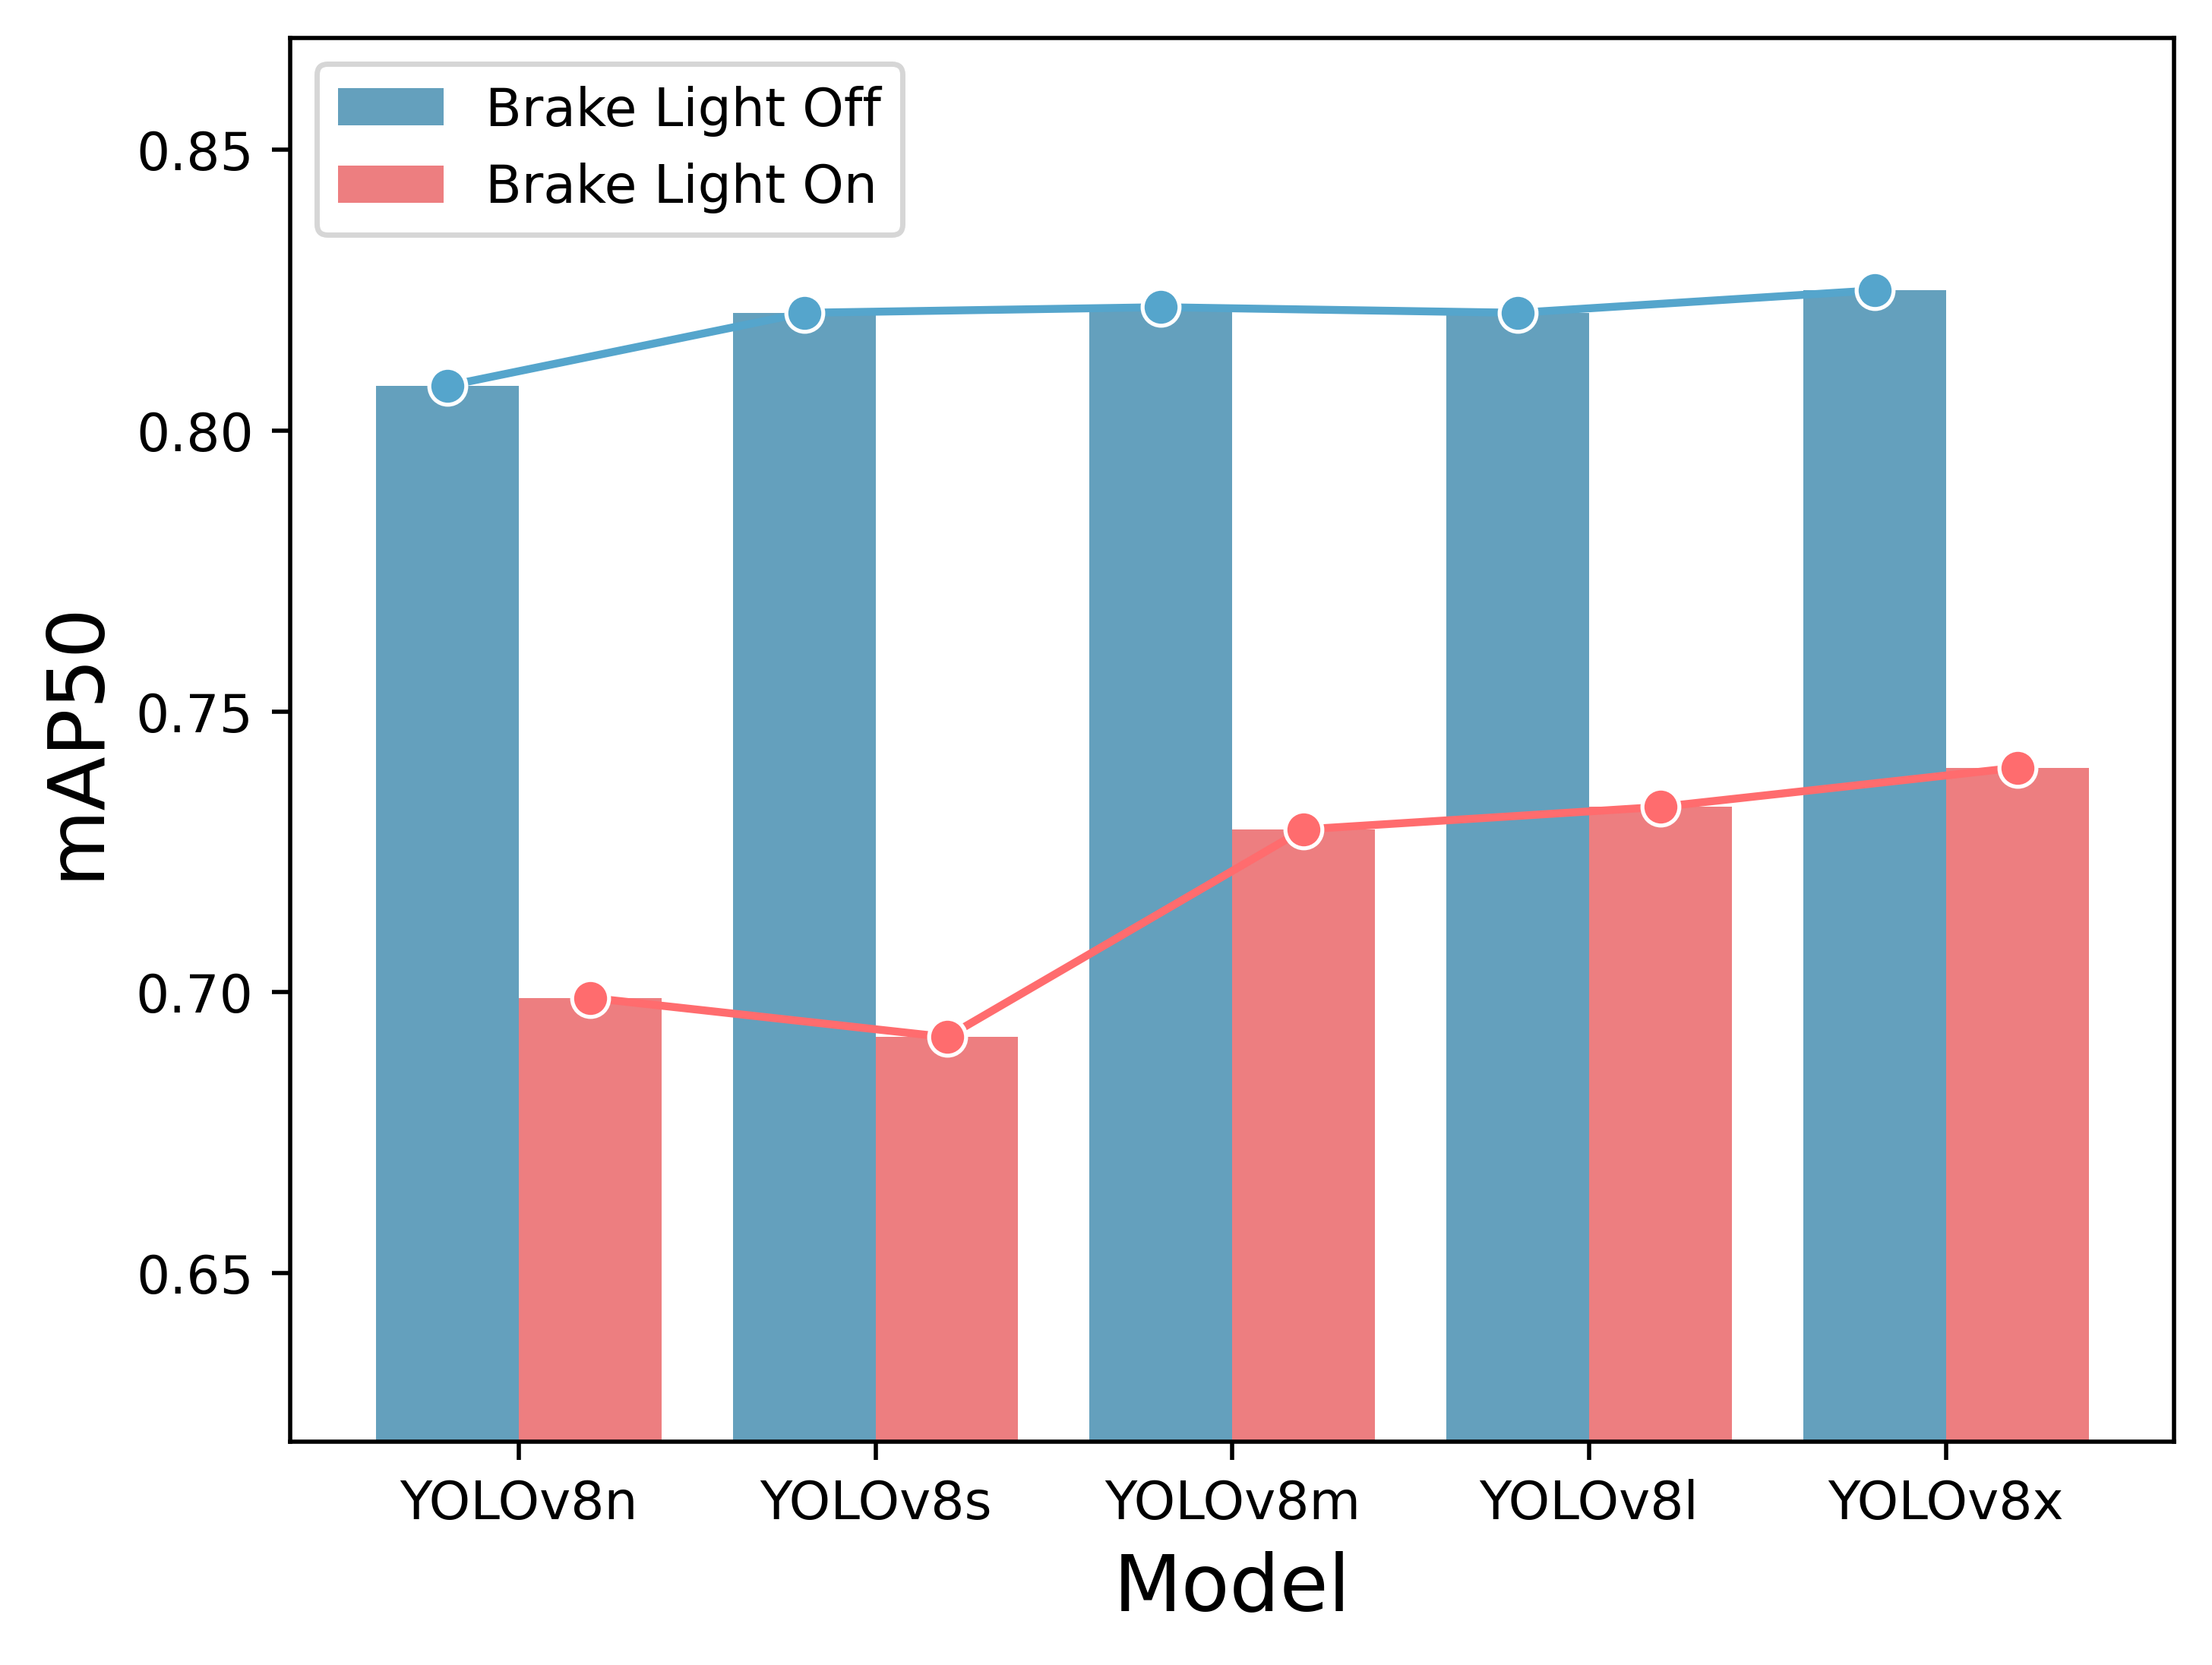
\includegraphics[height=5cm]{fig/bar_day_map50.png} }}%
    \subfloat[mAP50 on the Night testset]{{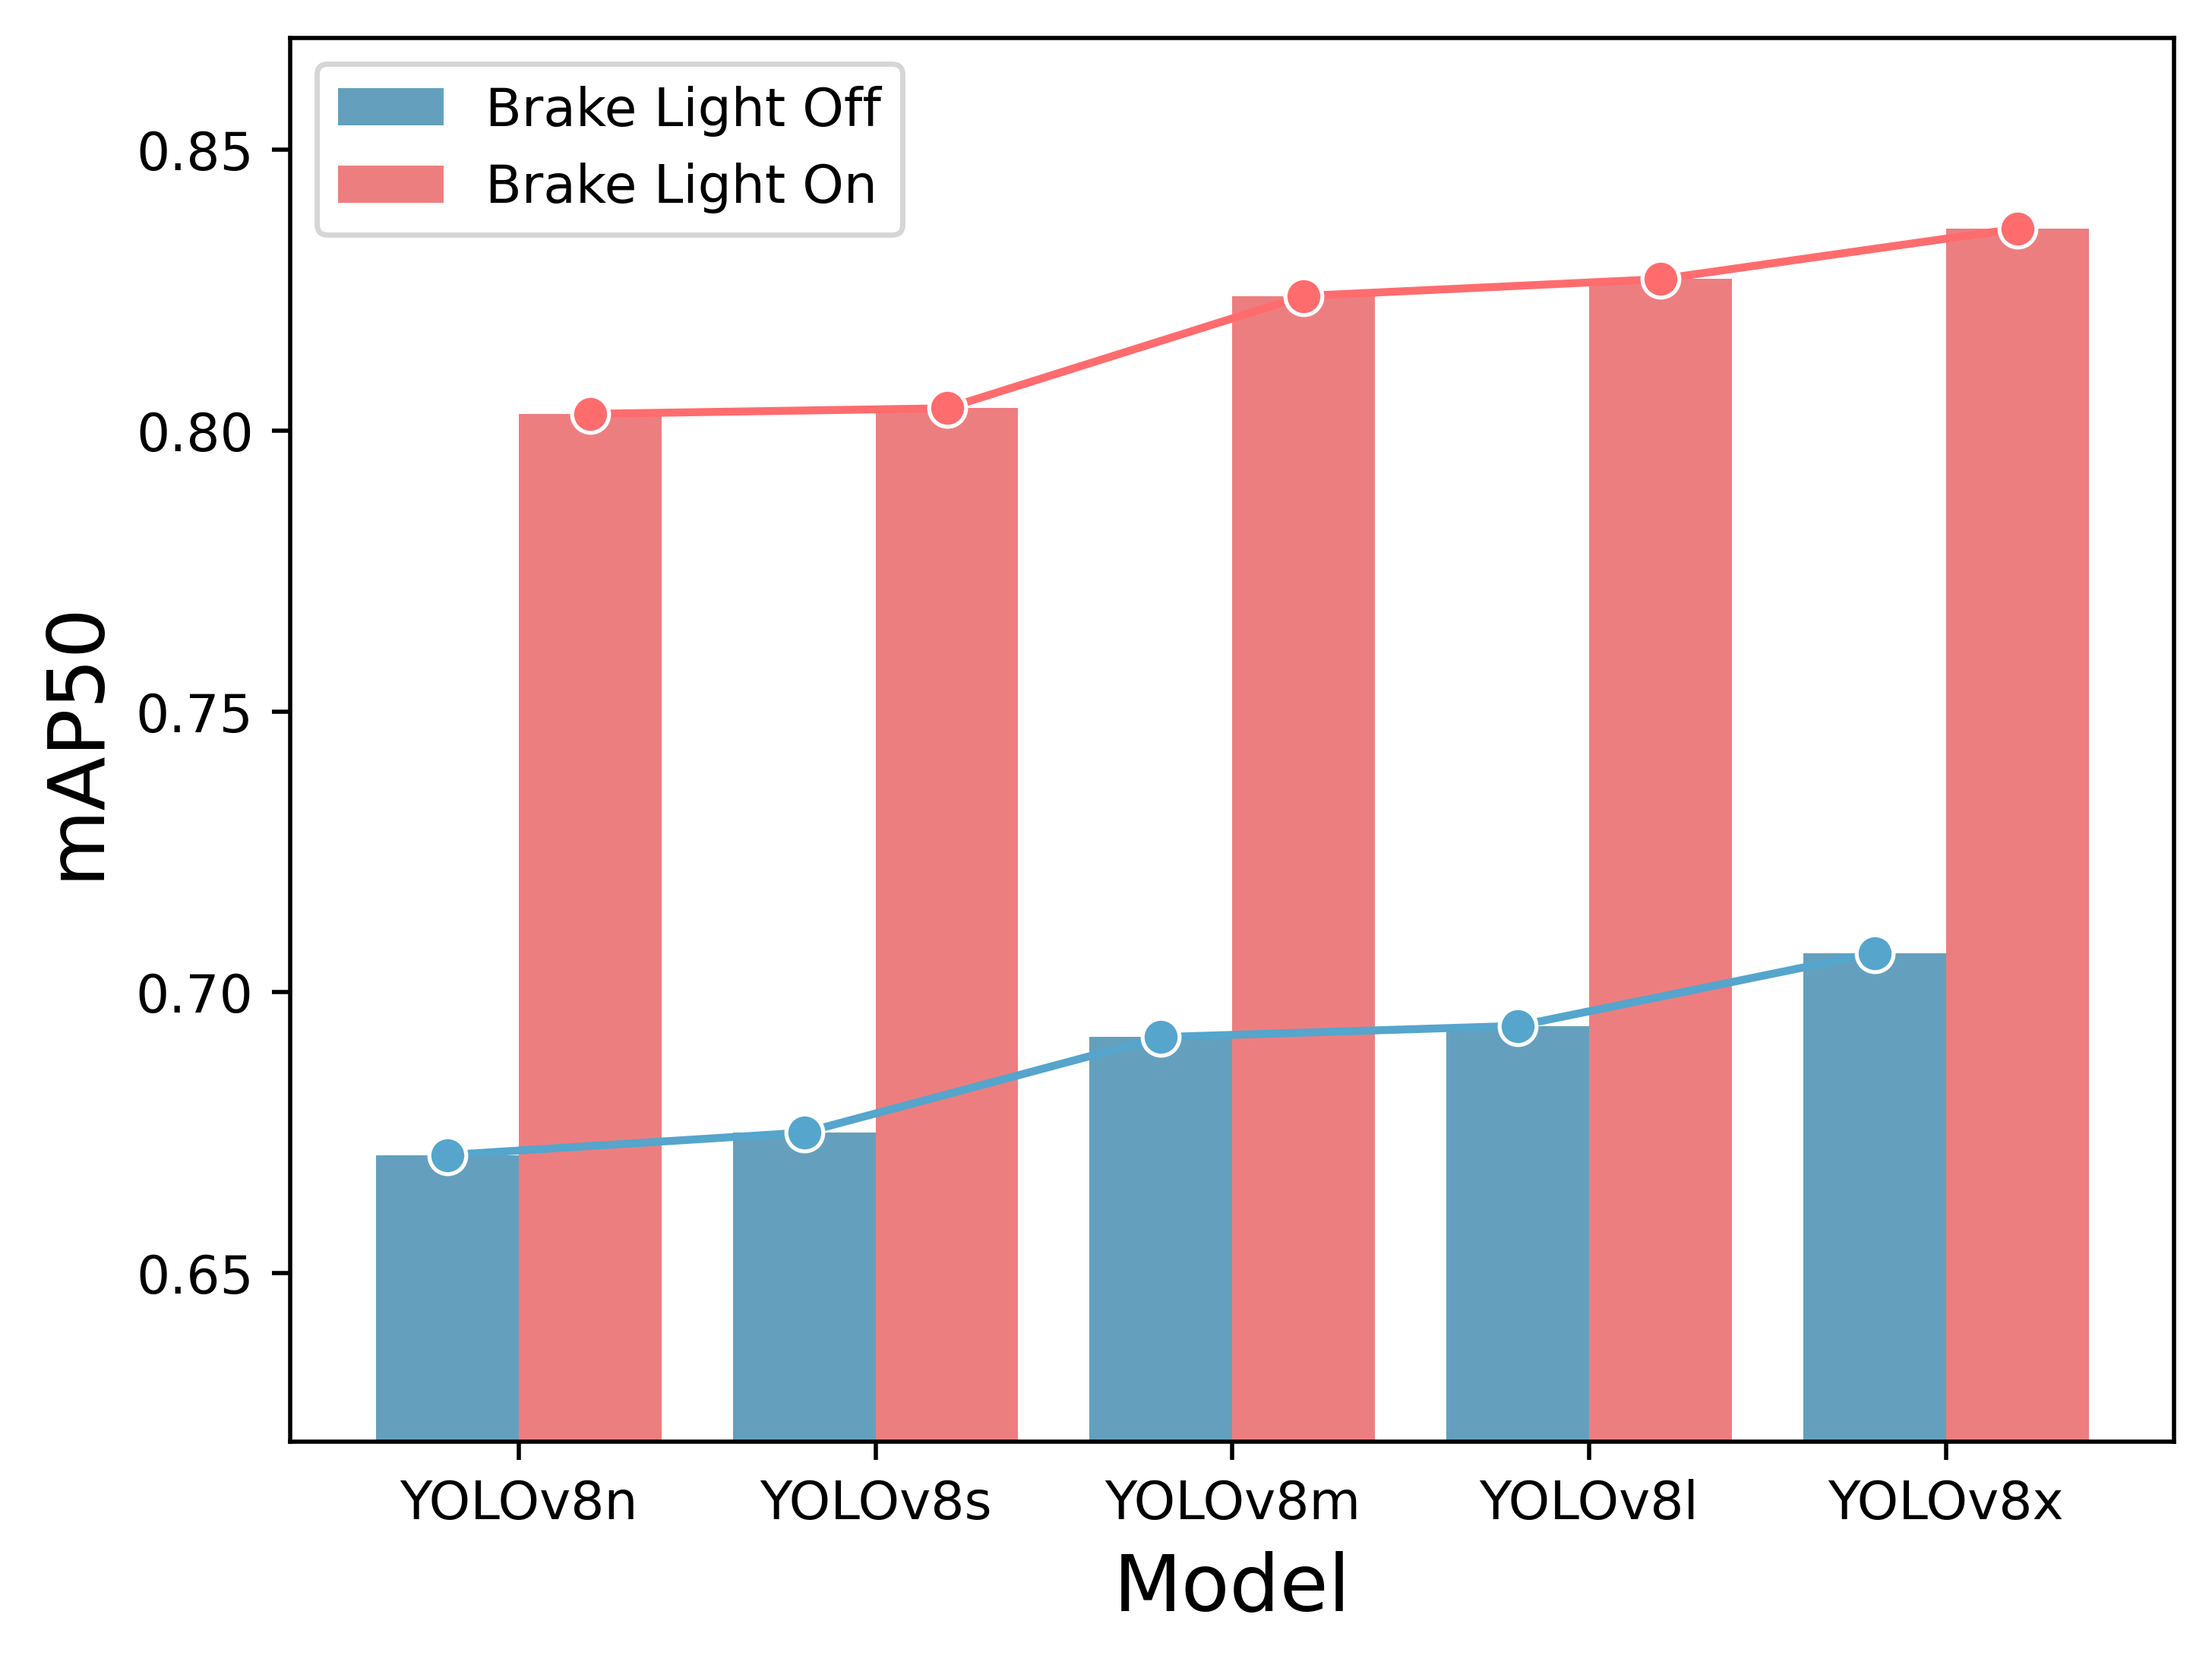
\includegraphics[height=5cm]{fig/bar_night_map50.png} }}%
    \hfill
    \subfloat[mAP50-95 on the Day testset]{{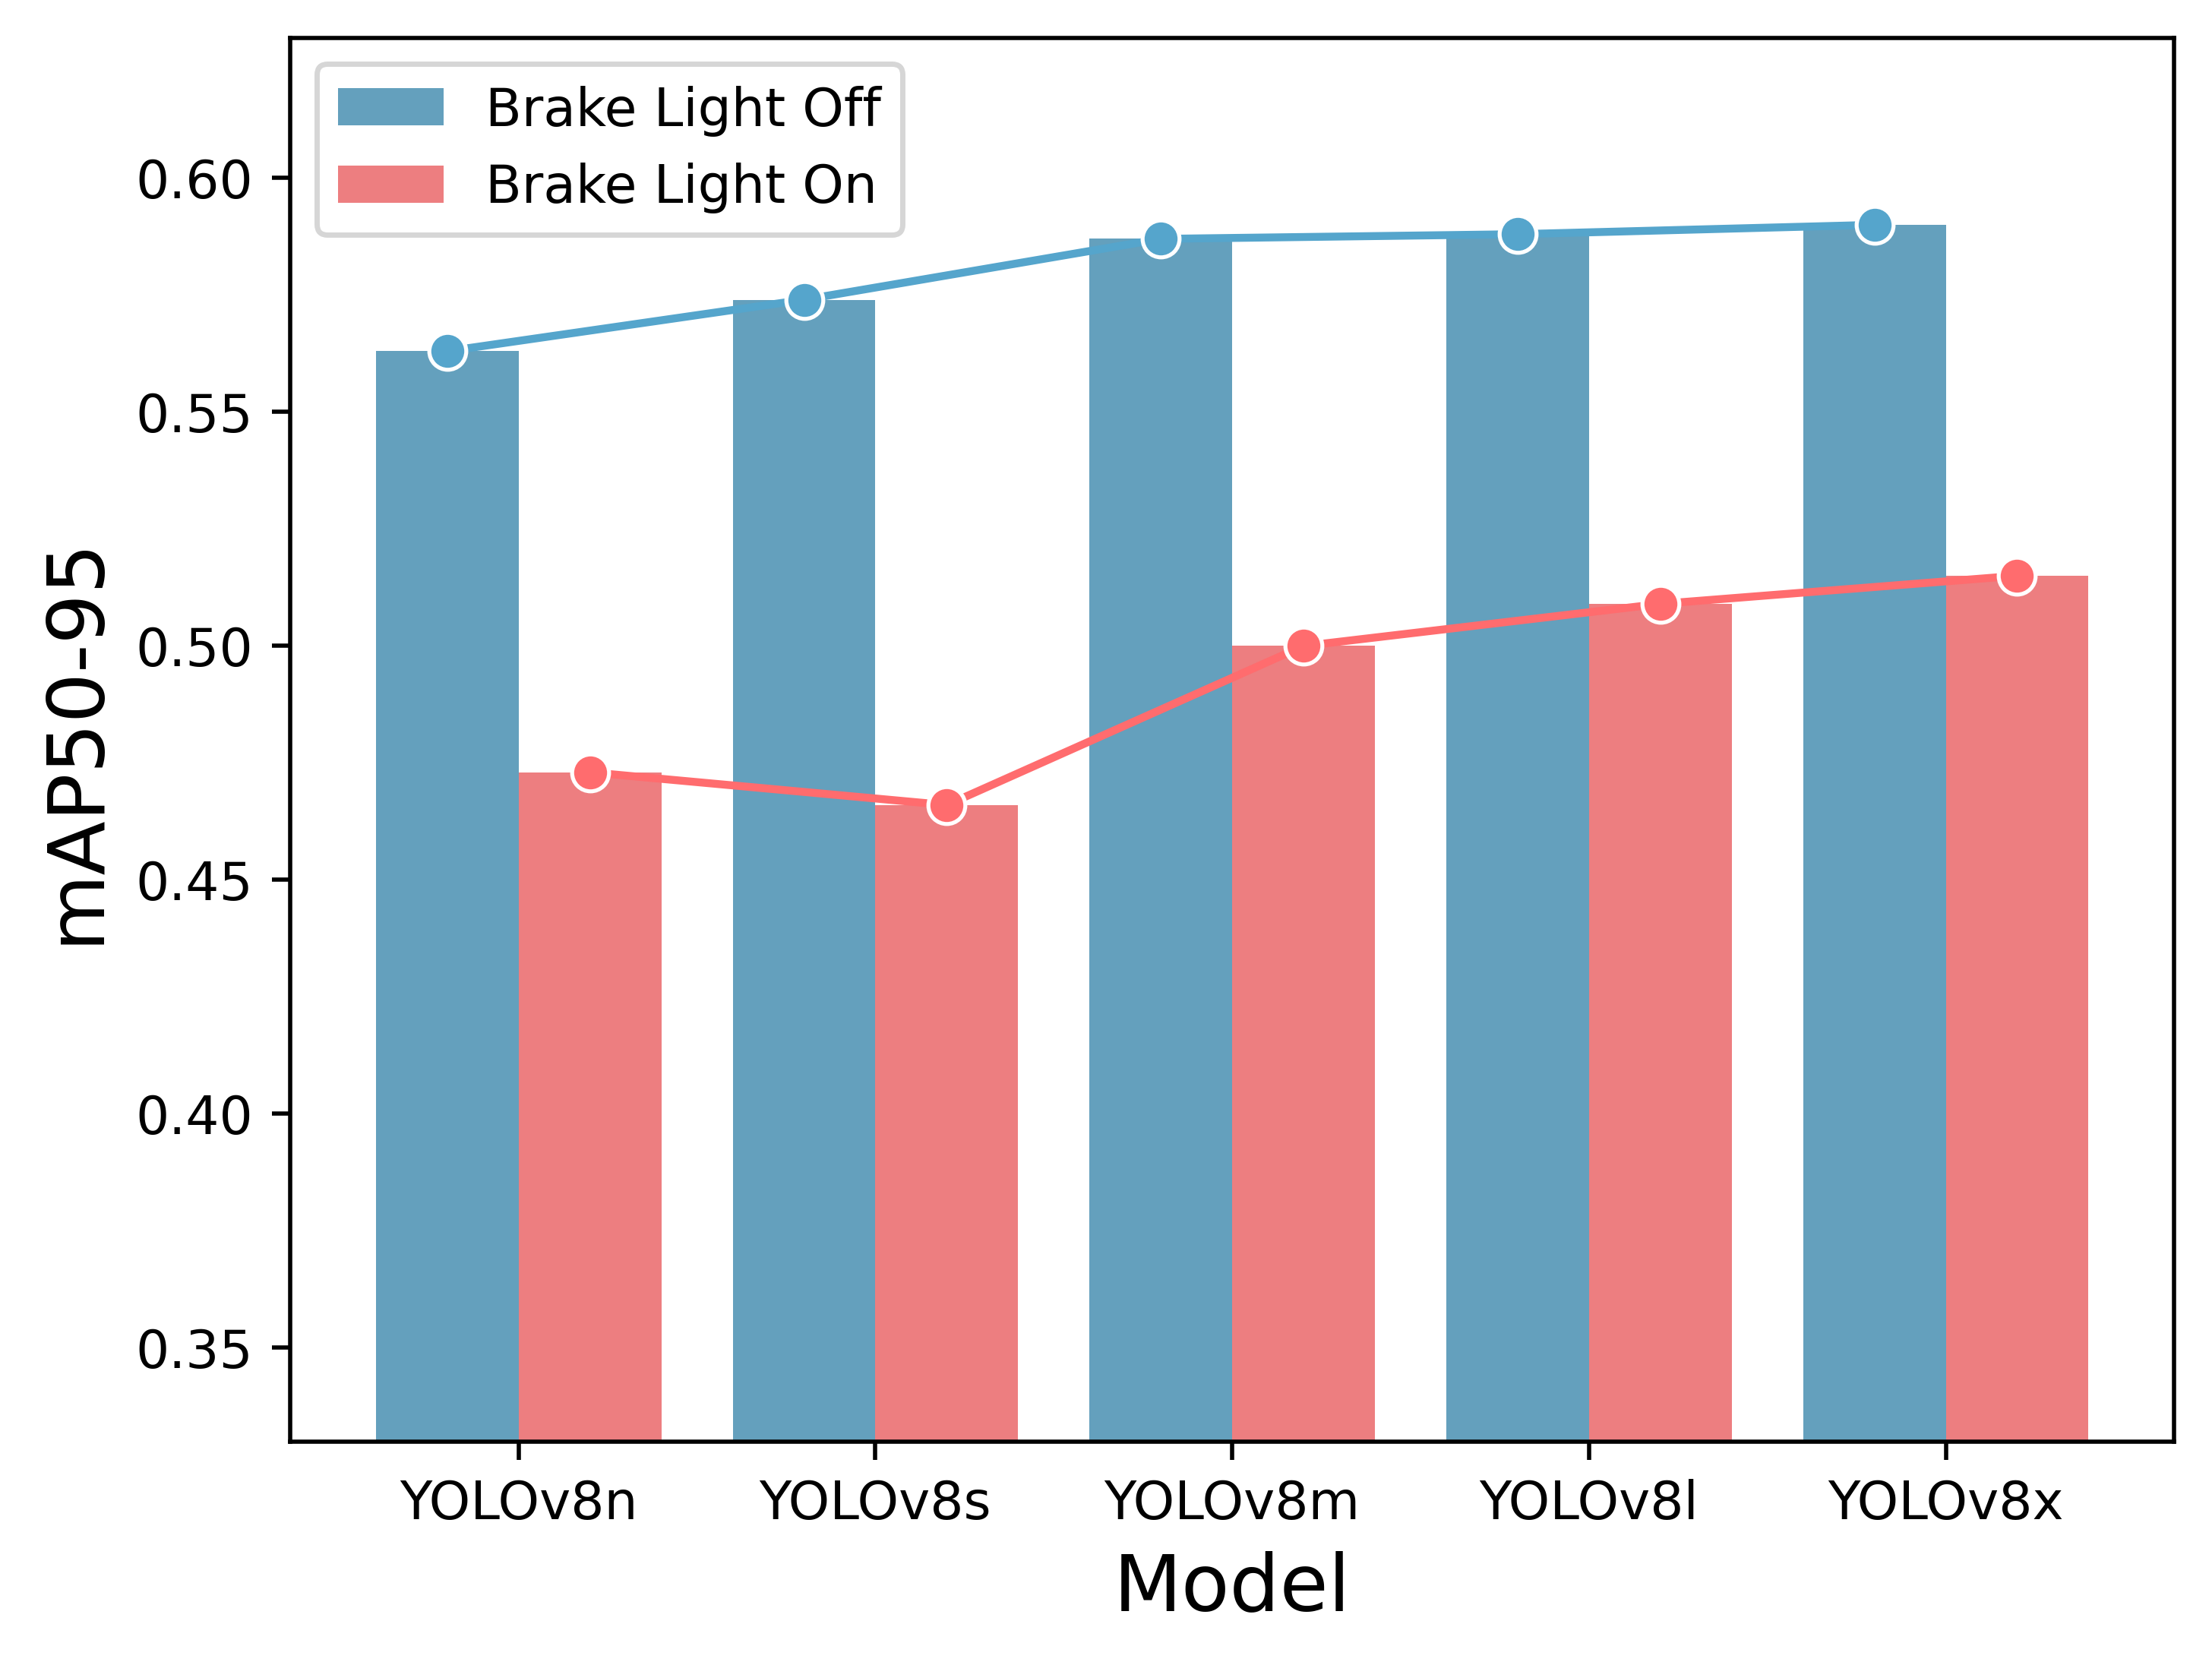
\includegraphics[height=5cm]{fig/bar_day_map50-95.png} }}%
    \subfloat[mAP50-95 on the Night testset]{{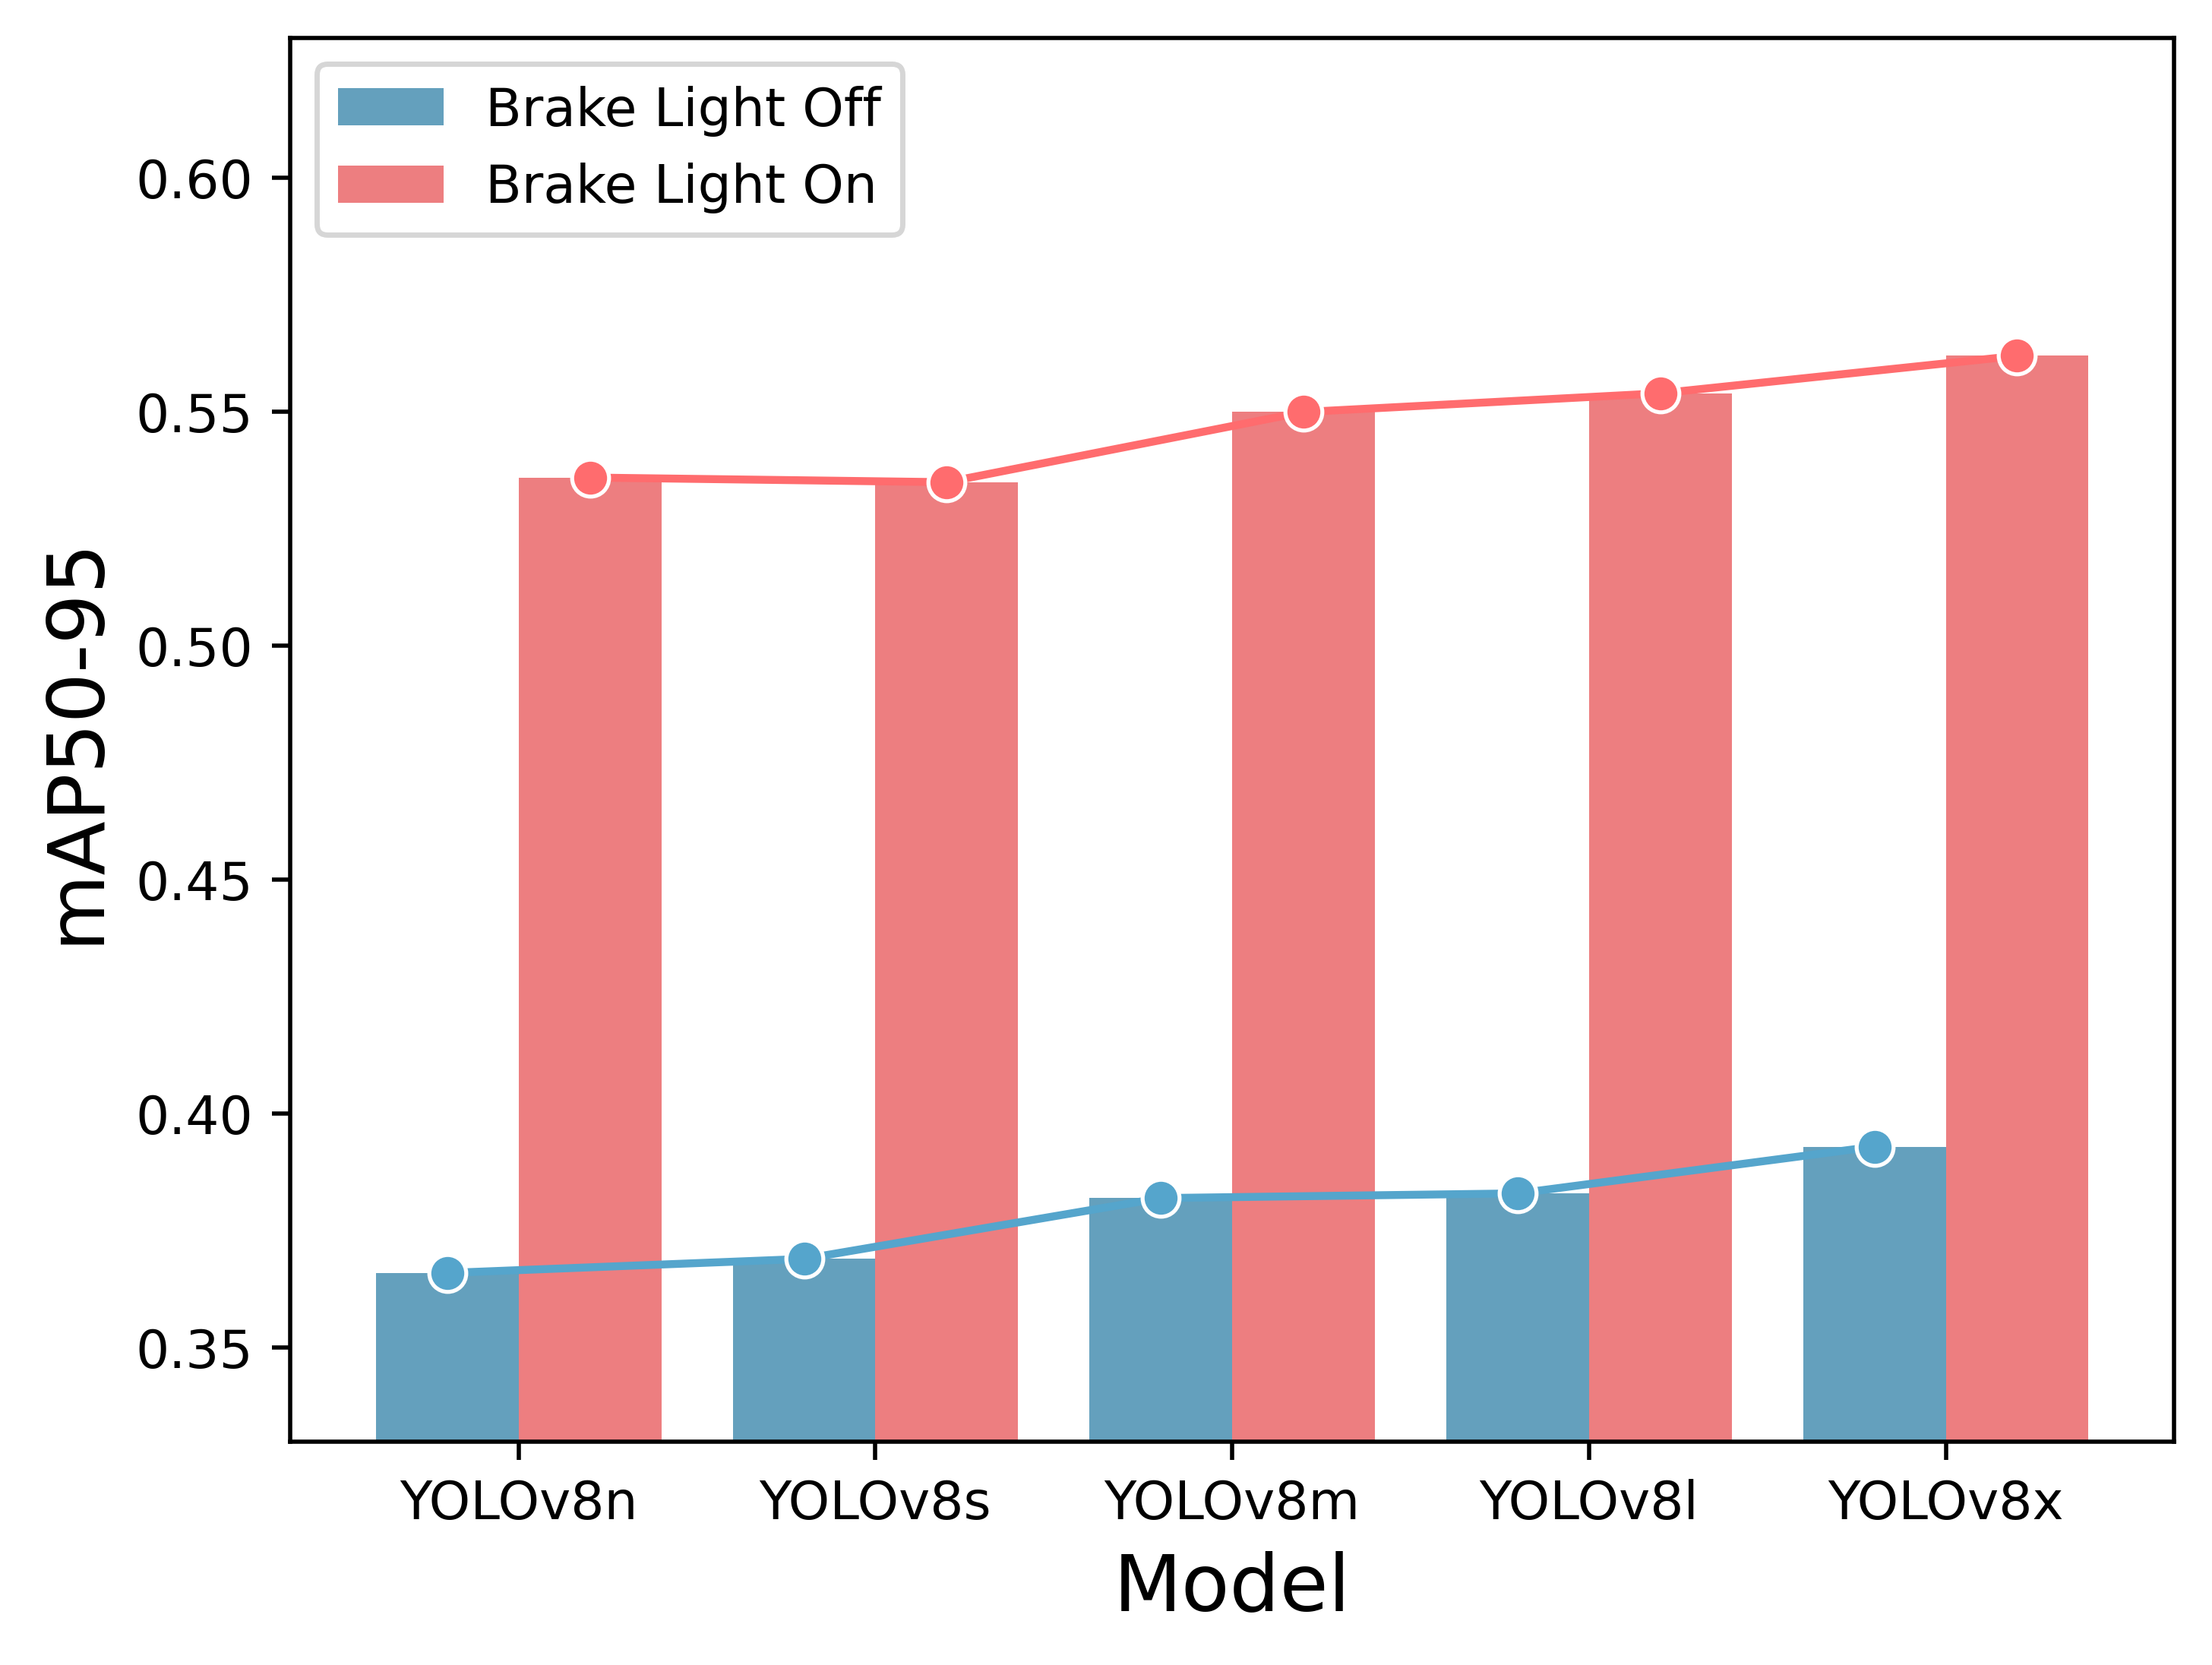
\includegraphics[height=5cm]{fig/bar_night_map50-95.png} }}%

\caption{Detection performance comparison for ambient illumination difference. The y-axis and x-axis represent the detection accuracy and lists the YOLOv8 models, respectively. Each model is depicted with two bars, showcasing the detection performance for brake light off and brake light on classes. Each line plots highlights the difference in detection performance by models for each class.}
\label{fig:dayNnight}%
\end{figure}

Figure \ref{fig:dayNnight} depicts the detection performance for each class on the Day/Night split test dataset. 
In Figure \ref{fig:dayNnight}-(a) and (b), mAP50 is plotted, while in Figure \ref{fig:dayNnight}-(c) and (d), mAP50-95 is plotted.
Figure \ref{fig:dayNnight}-(a) and (c) show the performance on the Day testset, while (b) and (d) show the performance on the Night testset.
On the Day testset, the detection performance for the brake light off class is better than that for the brake light on class.
Conversely, on the Night testset, the detection performance for the brake light on class is superior to that for the brake light off class.
The brake light off class, which was well detected in an environment with high ambient light, experienced a decline in detection performance as the ambient light decreased.
On the other hand, the brake light on class, which initially exhibited relatively low detection performance in an environment with high ambient light, demonstrated high detection performance when the ambient light was low.
The difference in performance due to ambient illumination is more pronounced in the brake light off class.
Detailed detection performance comparisons for ambient illumination difference for each model and class can be found in Table \ref{tab:dayNnight}.


\begin{table}[!h]
    \caption{Results of comparison for ambient illumination difference}
    \label{tab:dayNnight}
    % \resizebox{\textwidth}{!}{%
    \renewcommand{\arraystretch}{0.94}
    \begin{tabular}{llcccc}
    \toprule
    \multicolumn{1}{c}{\multirow{2}{*}{Model}} & \multicolumn{1}{c}{\multirow{2}{*}{Class}} & \multicolumn{2}{c}{mAP50}                           & \multicolumn{2}{c}{mAP50-95}                        \\
    \multicolumn{1}{c}{}                       & \multicolumn{1}{c}{}                       & \multicolumn{1}{c}{Day} & \multicolumn{1}{c}{Night} & \multicolumn{1}{c}{Day} & \multicolumn{1}{c}{Night} \\
    \midrule
    \multirow{3}{*}{YOLOv8n}                   & Brake Light Off                            & 0.808          & 0.671               & 0.563          & 0.366                     \\
    & Brake Light On                             & 0.699                   & 0.803            & 0.473                   & 0.536            \\
    & \multicolumn{1}{r}{Total}                  & 0.753          & 0.737                     & 0.518          & 0.451                     \\

    \midrule
    \multirow{3}{*}{YOLOv8s}                   & Brake Light Off                            & 0.821          & 0.675                     & 0.574          & 0.369                     \\
    & Brake Light On                             & 0.692                   & 0.804            & 0.466                   & 0.535            \\
    & \multicolumn{1}{r}{Total}                  & 0.757          & 0.739                     & 0.520          & 0.452                     \\

    \midrule
    \multirow{3}{*}{YOLOv8m}                   & Brake Light Off                            & 0.822          & 0.692                     & 0.587          & 0.382                     \\
    & Brake Light On                             & 0.729                   & 0.824            & 0.500                   & 0.550            \\
    & \multicolumn{1}{r}{Total}                  & 0.776                   & 0.758                     & 0.544          & 0.466                     \\

    \midrule
    \multirow{3}{*}{YOLOv8l}                   & Brake Light Off                            & 0.821          & 0.694                     & 0.588          & 0.383                     \\
                                           & Brake Light On                             & 0.733                   & 0.827            & 0.509                   & 0.554            \\
                                           & \multicolumn{1}{r}{Total}                  & 0.777          & 0.761                     & 0.549          & 0.468                    \\
    \midrule
    \multirow{3}{*}{YOLOv8x}                   & Brake Light Off                            & 0.825          & 0.707                     & 0.590          & 0.393                     \\
                                           & Brake Light On                             & 0.740                   & 0.836            & 0.515                   & 0.562            \\
                                           & \multicolumn{1}{r}{Total}                  & 0.782          & 0.772                     & 0.552          & 0.477                    \\
    \bottomrule
    \end{tabular}%
    % }
\end{table}



According to the detailed analysis, the performance difference attributed to the difference in ambient illumination can be explained in terms of accuracy.
The overall accuracies for driving vehicle detection across all classes were $0.87$ in the Day testset and $0.89$ in the Night testset.
As the ambient illumination decreased, the accuracy for driving vehicle detection slightly improved.
However, the accuracies for the brake light off class decreased to $0.67$ in the Day testset and $0.43$ in the Night testset, while the accuracies for the brake light on class increased to $0.75$ in the Day testset and $0.86$ in the Night testset.
The detailed analysis revealed that this performance difference is influenced by the presence of tail lights.
% , the cause of the difference in performance due to the difference in ambient illumination is represented by two factors.
% Therefore, as the ambient illumination decreases, the overall detection performance for driving vehicles improves, while the detection performance for the brake light off class deteriorates and the performance for the brake light on class improves.
% We argue that this phenomenon is influenced by the tail light.
As the ambient illumination decreases, the tail lights of the vehicles are turned on, enhancing the detection performance for driving vehicles.
However, the turned-on tail lights can cause confusion with the turned-on brake lights, leading to a decreases in the detection performance for brake light off class.
Consequently, the decrease in ambient illumination improves the detection performance of vehicles with the brake light turned on while deteriorating the detection performance of vehicles with the brake light turned off.


\begin{figure}[!t]
    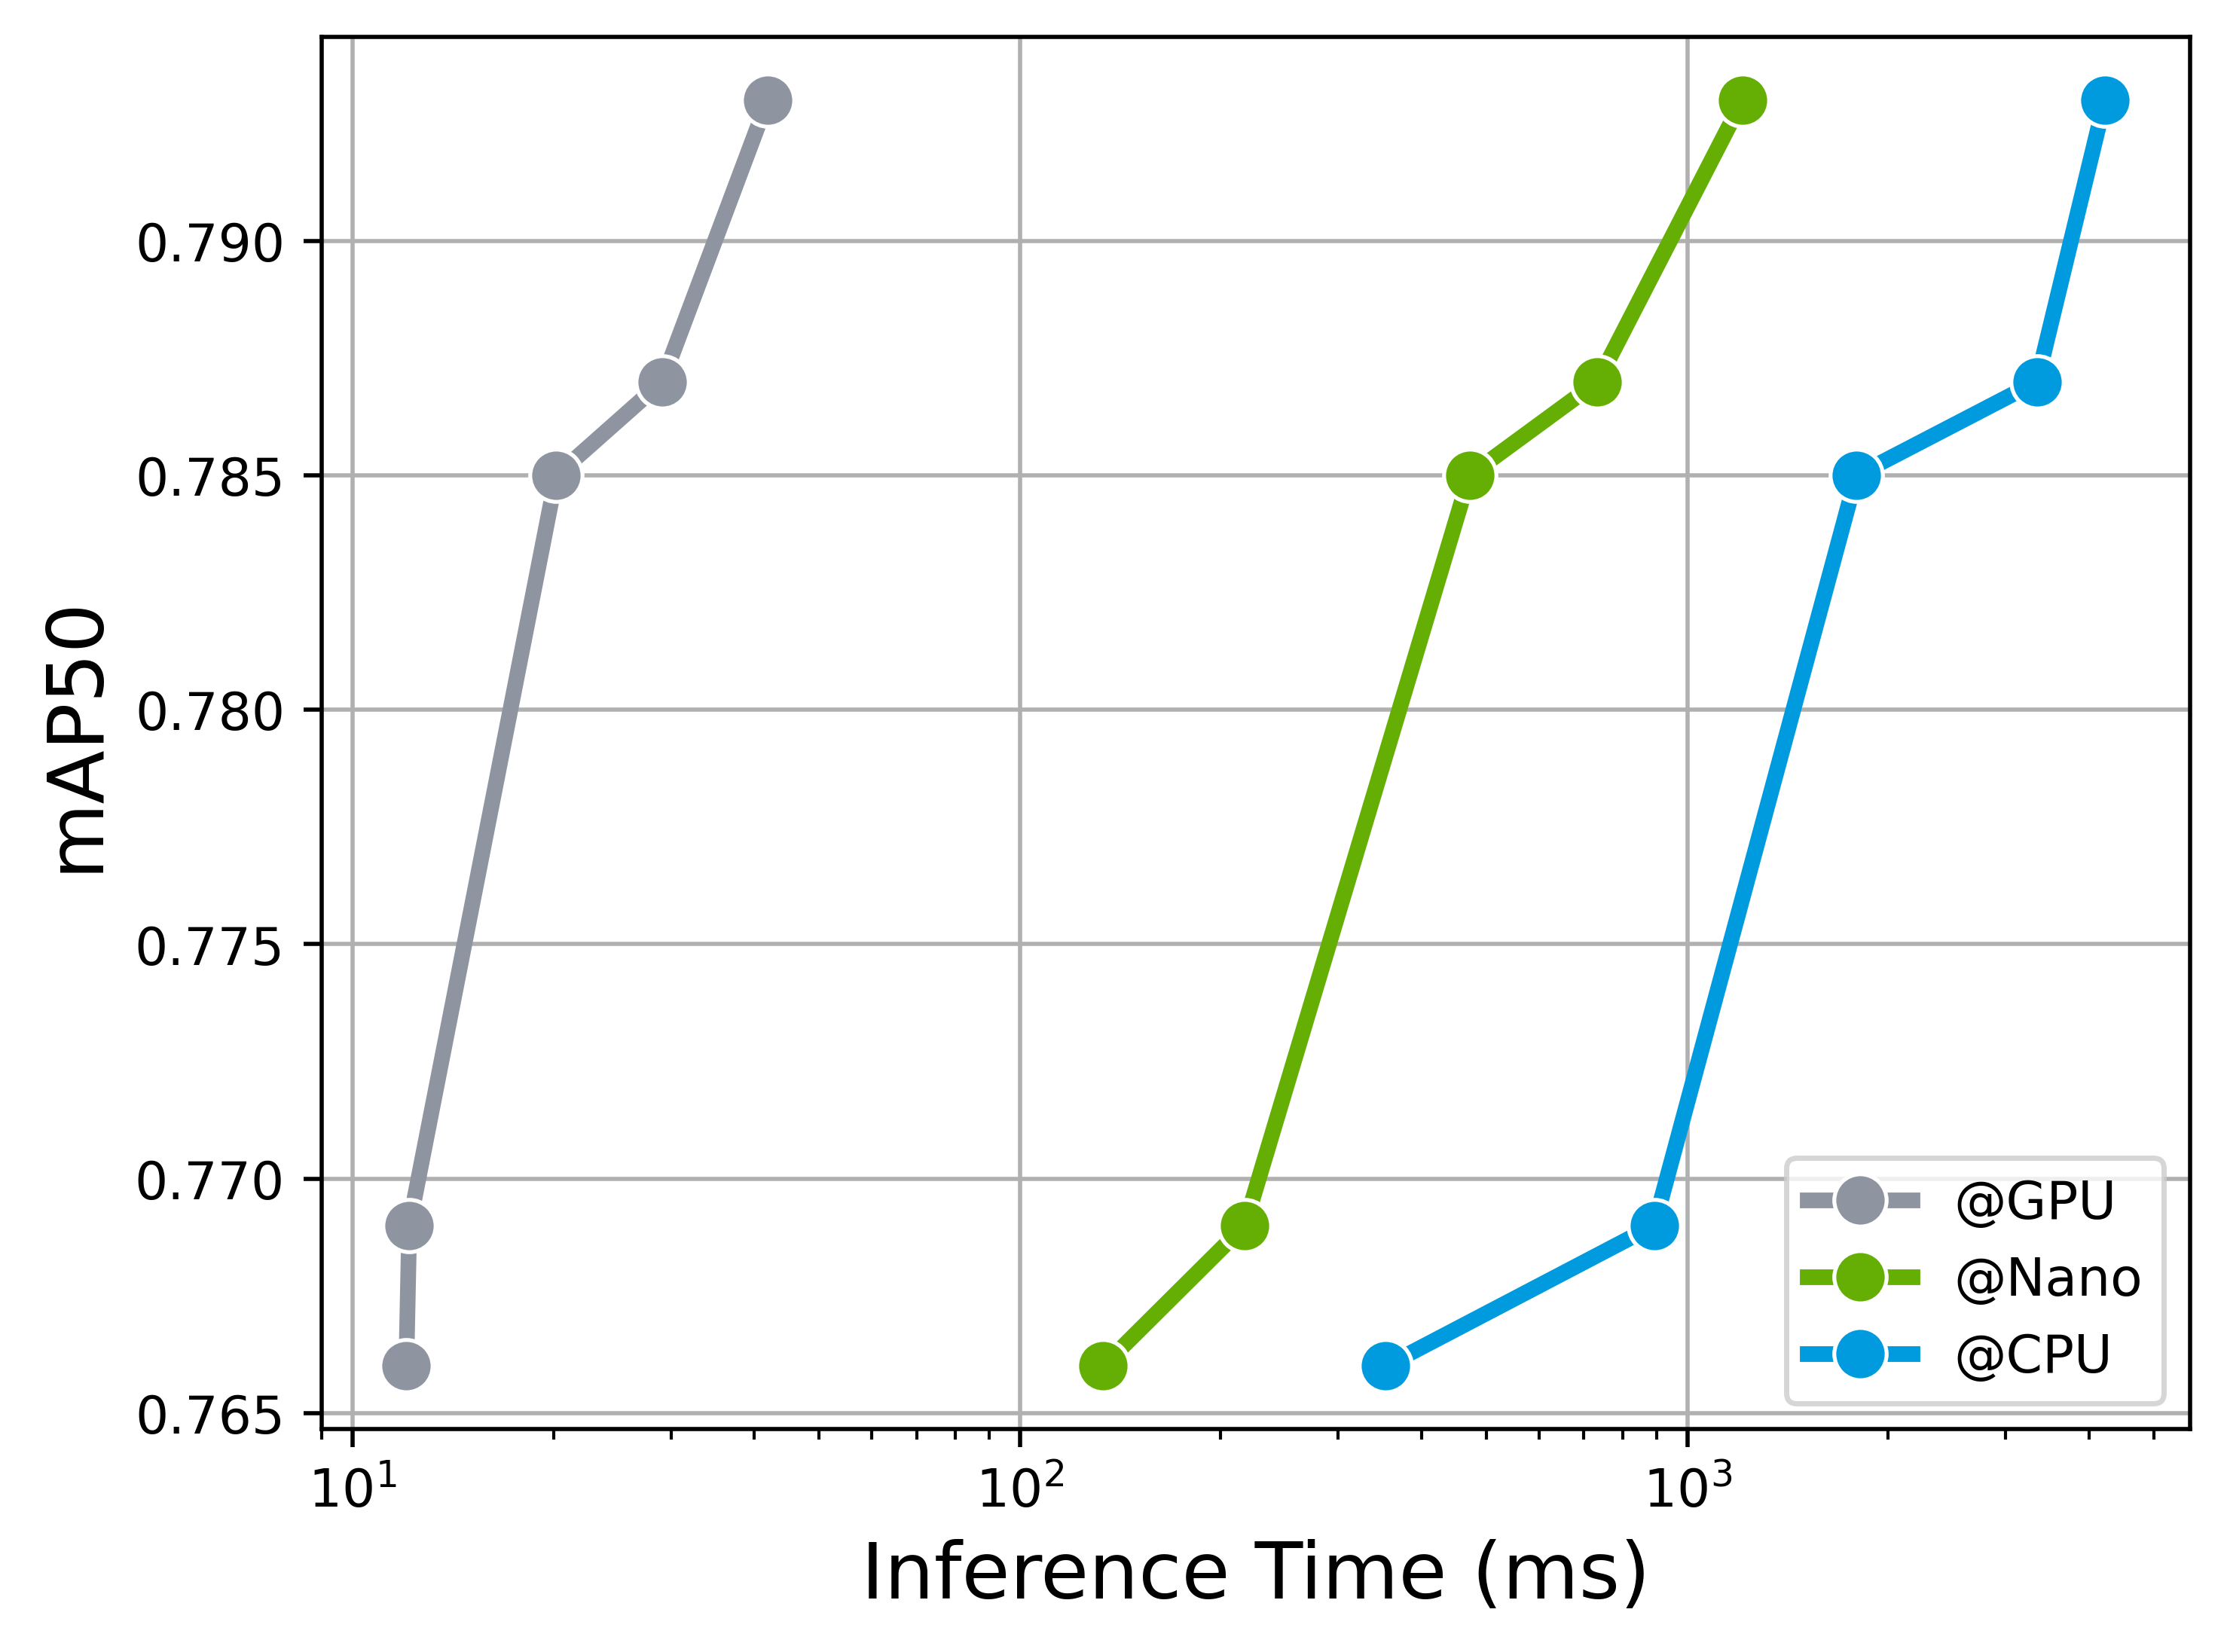
\includegraphics[scale=0.5]{fig/plot_inference_time.png}
    \caption{Trade-off between inference time and detection accuracy in different environments. The x-axis represents the inference time and the y-axis represents the detection accuracy as mAP50. It showcases the trends in inference speed and detection performance for differenct sizes of YOLOv8 under different computing environments as follows: ``@GPU'' refers to Nvidia Tesla T4, ``@Nano'' refers to Nvidia Jetson Nano, and ``@CPU'' refers to Intel Xeon processor.}
    \label{fig:inference}
\end{figure}

\begin{table}[!b]
    \caption{Results of comparison for inference time in different environments. All models were inferred by converting to ONNX form, and the different computing environments are as follows: ``@GPU'' refers to Nvidia Tesla T4, ``@Nano'' refers to Nvidia Jetson Nano, and ``@CPU'' refers to Intel Xeon processor.}
    \label{tab:inference}
    \begin{tabular}{lrrr}
    \toprule
    \multicolumn{1}{c}{\multirow{2}{*}{Model}}   & \multicolumn{3}{c}{Inference Time (ms)} \\
                                 & ONNX @GPU & ONNX @Nano & ONNX @CPU \\
    \midrule
    YOLOv8n & 12.04        & 133.30            & 353.13    \\
    YOLOv8s & 12.16        & 217.20            & 891.93    \\
    YOLOv8m & 20.20        & 471.59            & 1,792.31   \\
    YOLOv8l & 29.09       & 733.27            & 3,340.26   \\
    YOLOv8x & 41.87       & 1,208.69           & 4,222.87  \\
    \bottomrule
    \end{tabular}%
\end{table}

In order to validate the real-time inference performance of the trained models on edge devices, experiments were conducted to evaluated both accurate detection and inference time. 
The Nvidia Jetson Nano device was utilized for this perpose.
The trained models were converted to the Open Neural Network Exchange (ONNX) format, which is an open format that facilitates the sharing and interoperability of neural network models across different frameworks. The inference time was measured on the Jetson Nano device using the ONNX models.
The measured inference times ranged from $133.30$ ms to $733.27$ ms, depending on the size of the model.
Considering that brake light status detection is a perception algorithm and JetSon Nano is sufficiently rigorous for testing real-time performance, the achieved inference time of $133.30$ ms with the smallest model, the YOLOv8n, can be considered sufficiently real-time.
The trade-off performance between inference time and detection accuracy is illustrated in Figure \ref{fig:inference}.
To provide a comprehensive performance comparison, the performance on different devices, including the Jetson Nano, CPU (Intel Xeon 2.20GHz), and GPU (Nvidia Tesla T4), was included.
Detailed values can be found in Table \ref{tab:inference}.



